%%%%%%%%%%%%%%%%%%%%%%%%%%%%%%%%%%%%%%%%%%%%%%%%%%%%%%%%%%%%%%%%%%%%%
%% This is a (brief) model paper using the achemso class
%% The document class accepts keyval options, which should include
%% the target journal and optionally the manuscript type. 
%%%%%%%%%%%%%%%%%%%%%%%%%%%%%%%%%%%%%%%%%%%%%%%%%%%%%%%%%%%%%%%%%%%%%
\documentclass[journal=jacsat,manuscript=article]{achemso}
\SectionNumbersOn
\usepackage{tikz} %Format quantum circuits
\usetikzlibrary{quantikz2}%Format quantum circuits

\usepackage{multicol}
\usepackage{graphicx}% Include figure files
\usepackage{graphicx}% Include figure files
\usepackage{dcolumn}% Align table columns on decimal point
\usepackage{bm}% bold math
%\usepackage[mathlines]{lineno}% Enable numbering of text and display math
%\linenumbers\relax % Commence numbering lines
\usepackage{pgffor}
\usepackage[utf8]{inputenc}
\usepackage[T1]{fontenc}
\usepackage{mathptmx}
\usepackage{listings}
\lstset{language=Python}
\usepackage{rotating} % Rotating table
\usepackage{caption}
\usepackage{subcaption}

\usepackage{color}
\usepackage{dcolumn} % decimal align in tables
\usepackage{bm} % bold math
\usepackage{graphicx}
\usepackage{multirow} % for table cells to span rows
\usepackage{pifont} % for checkmarks
\usepackage{epsfig}
\usepackage{amsmath} % matrix
% \usepackage{subfigure}
\usepackage{float}
\usepackage{booktabs}
\usepackage{tabularx}
\usepackage{natbib}
\usepackage{gensymb}
\setlength{\paperwidth}{8.5in}
\setlength{\paperheight}{11.0in}
\usepackage{rotating}
\usepackage{threeparttable}
\usepackage{comment}
%for corrections
\usepackage[normalem]{ulem}
\usepackage[hidelinks]{hyperref} % allows hyperlinking for references
%%%%%%%%%%%%%%%%%%%%%%%%%%%%%%%%%%%%%%%%%%%%%%%%%%%%%%%%%%%%%%%%%%%%%
%% Place any additional packages needed here.  Only include packages
%% which are essential, to avoid problems later. Do NOT use any
%% packages which require e-TeX (for example etoolbox): the e-TeX
%% extensions are not currently available on the ACS conversion
%% servers.
%%%%%%%%%%%%%%%%%%%%%%%%%%%%%%%%%%%%%%%%%%%%%%%%%%%%%%%%%%%%%%%%%%%%%
\usepackage[version=3]{mhchem} % Formula subscripts using \ce{}
\usepackage{xcolor}
\usepackage{amsmath,amssymb,amsthm}
\usepackage{mathtools,physics}
\usepackage{subcaption}
% \usepackage{titling}
%%%%%%%%%%%%%%%%%%%%%%%%%%%%%%%%%%%%%%%%%%%%%%%%%%%%%%%%%%%%%%%%%%%%%
%% If issues arise when submitting your manuscript, you may want to
%% un-comment the next line.  This provides information on the
%% version of every file you have used.
%%%%%%%%%%%%%%%%%%%%%%%%%%%%%%%%%%%%%%%%%%%%%%%%%%%%%%%%%%%%%%%%%%%%%
%%\listfiles

%%%%%%%%%%%%%%%%%%%%%%%%%%%%%%%%%%%%%%%%%%%%%%%%%%%%%%%%%%%%%%%%%%%%%
%% Place any additional macros here.  Please use \newcommand* where
%% possible, and avoid layout-changing macros (which are not used
%% when typesetting).
%%%%%%%%%%%%%%%%%%%%%%%%%%%%%%%%%%%%%%%%%%%%%%%%%%%%%%%%%%%%%%%%%%%%%
\newtheorem{theorem}{Theorem}[section]
\newtheorem{corollary}{Corollary}
\newtheorem{lemma}[theorem]{Lemma}
\newtheorem{proposition}{Proposition}
\newtheorem{conjecture}{Conjecture}
\newtheorem{definition}[theorem]{Definition}
\newtheorem{assumption}[theorem]{Assumption}
% \newtheorem{example}[theorem]{Example}
\newtheorem{example}{Example}[section]
\newtheorem{remark}{Remark}

% Add line numbers, as requested by Nature
\usepackage{lineno}
% \linenumbers


\newcommand*\mycommand[1]{\texttt{\emph{#1}}}
\newcommand{\noteg}[1]{\textcolor{red}{({Grier: #1})}}
\newcommand{\notek}[1]{\textcolor{darkspringgreen}{({Kostas: #1})}}

\def\myvdots{\ \vdots\ }
%%%% HELPER CODE FOR DEALING WITH EXTERNAL REFERENCES
% (from an answer by cyberSingularity at http://tex.stackexchange.com/a/69832/226)
%%%

\usepackage{xr-hyper}
%%%%%%%%%%%%%%%%%%%%%%%%%%%%%%%%%%%%%%%%%%%%%%%%%%%%%%%%%%%%%%%%%%%%%%%%
%----Helper code for dealing with external references----
% (by cyberSingularity at http://tex.stackexchange.com/a/69832/226)

\usepackage{xr}
\makeatletter

\newcommand*{\addFileDependency}[1]{% argument=file name and extension
\typeout{(#1)}% latexmk will find this if $recorder=0
% however, in that case, it will ignore #1 if it is a .aux or 
% .pdf file etc and it exists! If it doesn't exist, it will appear 
% in the list of dependents regardless)
%
% Write the following if you want it to appear in \listfiles 
% --- although not really necessary and latexmk doesn't use this
%
\@addtofilelist{#1}
%
% latexmk will find this message if #1 doesn't exist (yet)
\IfFileExists{#1}{}{\typeout{No file #1.}}
}\makeatother

\newcommand*{\myexternaldocument}[1]{%
\externaldocument{#1}%
\addFileDependency{#1.tex}%
\addFileDependency{#1.aux}%
}
%------------End of helper code--------------

% put all the external documents here!
\myexternaldocument{SI}
\newcommand{\siref}[1]{S\ref{#1}}
%%%%%%%%%%%%%%%%%%%%%%%%%%%%%%%%%%%%%%%%%%%%%%%%%%%%%%%%%%%%%%%%%%%%%%%%


%%%%%%%%%%%%%%%%%%%%%%%%%%%%%%%%%%%%%%%%%%%%%%%%%%%%%%%%%%%%%%%%%%%%%
%% The document title should be given as usual. Some journals require
%% a running title from the author: this should be supplied as an
%% optional argument to \title.
%%%%%%%%%%%%%%%%%%%%%%%%%%%%%%%%%%%%%%%%%%%%%%%%%%%%%%%%%%%%%%%%%%%%%
\title{Understanding Parameterized Quantum Circuit Learning for Quantum Chemical Applications}
%%%%%%%%%%%%%%%%%%%%%%%%%%%%%%%%%%%%%%%%%%%%%%%%%%%%%%%%%%%%%%%%%%%%%
%% Meta-data block
%% ---------------
%% Each author should be given as a separate \author command.
%%
%% Corresponding authors should have an e-mail given after the author
%% name as an \email command. Phone and fax numbers can be given
%% using \phone and \fax, respectively; this information is optional.
%%
%% The affiliation of authors is given after the authors; each
%% \affiliation command applies to all preceding authors not already
%% assigned an affiliation.
%%
%% The affiliation takes an option argument for the short name.  This
%% will typically be something like "University of Somewhere".
%%
%% The \altaffiliation macro should be used for new address, etc.
%% On the other hand, \alsoaffiliation is used on a per author basis
%% when authors are associated with multiple institutions.
%%%%%%%%%%%%%%%%%%%%%%%%%%%%%%%%%%%%%%%%%%%%%%%%%%%%%%%%%%%%%%%%%%%%%
\author{Grier M. Jones}
\affiliation[UTSG ECE]{
The Edward S. Rogers Sr. Department of Electrical and Computer Engineering, 
University of Toronto, 
10 Kings College Road, Toronto, Ontario, 
Canada M5S 3G4}
\alsoaffiliation[UTM CHEM]{
Department of Chemical and Physical Sciences, 
University of Toronto Mississauga, 
3359 Mississauga Road, Mississauga, Ontario, 
Canada L5L 1C6}

\author{Nick Taylor}
\affiliation[UTSG ECE]{
The Edward S. Rogers Sr. Department of Electrical and Computer Engineering, 
University of Toronto, 
10 Kings College Road, Toronto, Ontario, 
Canada M5S 3G4}
          
\author{Viki Kumar Prasad}
\affiliation[UTSG ECE]{
The Edward S. Rogers Sr. Department of Electrical and Computer Engineering, 
University of Toronto, 
10 Kings College Road, Toronto, Ontario, 
Canada M5S 3G4}
\alsoaffiliation[UTM CHEM]{
Department of Chemical and Physical Sciences, 
University of Toronto Mississauga, 
3359 Mississauga Road, Mississauga, Ontario, 
Canada L5L 1C6}
\alsoaffiliation[UT DSI]{
	Data Science Institute, 
	University of Toronto, 
	700 University Ave 10th floor,
	 Toronto, ON M7A 2S4}
\alsoaffiliation[UCalg]{Current Affiliation: Department of Chemistry, 
	University of Calgary, 
	2500 University Drive NW,
	 Calgary, AB T2N 1N4}





\author{Ulrich Fekl}
\affiliation[UTM CHEM]{
Department of Chemical and Physical Sciences, 
University of Toronto Mississauga, 
3359 Mississauga Road, Mississauga, Ontario, 
Canada L5L 1C6}
\email{ulrich.fekl@utoronto.ca}

\author{Hans-Arno Jacobsen}
\affiliation[UTSG ECE]{
The Edward S. Rogers Sr. Department of Electrical and Computer Engineering, 
University of Toronto, 
10 Kings College Road, Toronto, Ontario, 
Canada M5S 3G4}
\email{jacobsen@eecg.toronto.edu}
%%%%%%%%%%%%%%%%%%%%%%%%%%%%%%%%%%%%%%%%%%%%%%%%%%%%%%%%%%%%%%%%%%%%%
%% Some journals require a list of abbreviations or keywords to be
%% supplied. These should be set up here, and will be printed after
%% the title and author information, if needed.
%%%%%%%%%%%%%%%%%%%%%%%%%%%%%%%%%%%%%%%%%%%%%%%%%%%%%%%%%%%%%%%%%%%%%
\abbreviations{}
\keywords{American Chemical Society, \LaTeX}

%%%%%%%%%%%%%%%%%%%%%%%%%%%%%%%%%%%%%%%%%%%%%%%%%%%%%%%%%%%%%%%%%%%%%
%% The manuscript does not need to include \maketitle, which is
%% executed automatically.
%%%%%%%%%%%%%%%%%%%%%%%%%%%%%%%%%%%%%%%%%%%%%%%%%%%%%%%%%%%%%%%%%%%%%
\newcommand{\R}{\mathbb{R}}

\begin{document}

\section*{Abstract}
Within the quantum machine learning (QML) field, parameterized quantum circuits (PQCs), built using fixed and parameterized gates, offer a hybrid approach for complex machine learning tasks. While many potential use cases have been proposed, the exploration of relevant datasets for chemists is lacking. Our study seeks to understand the possible advantages and disadvantages of PQCs for two chemically relevant datasets: one based on the bond separation energies of 49 different classes of bonds, called the BSE49 dataset, and another consisting of water confirmations, where coupled-cluster singles and doubles (CCSD) wave functions are predicted using electronic structure theory data from lower-level methods using the data-driven coupled-cluster (DDCC) method. In our study, we examine a combinatorial space of 14 data encoding layers and 12 variational (ansatz) layers, for a combined total of 168 PQCs. To calibrate our PQCs, we utilize a dataset of noisy linear, quadratic, and sine functions to explore the effects of the circuit width and depth, the effects of the feature set size, and various error mitigation techniques. Following this step, we similarly examine our chemically relevant datasets. Our work highlights the difficulties in encoding classical molecular representations in a PQC for predicting bond separation energies and the aptitude for PQCs for predicting molecular wave functions. \par


\setcounter{secnumdepth}{1}
\section{Introduction}

In recent years, machine learning (ML) has emerged as a popular tool in chemistry for revealing new patterns in data, providing new insights beyond simple models and human experience, accelerating computations, and analyzing chemical space.
For computational chemists, the primary goal of applying ML is often to bypass the explicit calculation of molecular properties, which can be computationally expensive for large datasets.\cite{janet_machine_2020}
ML can be applied to a diverse set of applications including, but not limited to, accelerating molecular simulations\cite{behler_perspective_2016,ssmith_ani-1_2017,gao_torchani_2020}, determining molecular properties\cite{yang_analyzing_2019,ramakrishnan_quantum_2014,ramakrishnan_big_2015,hansen_machine_2015,unke_physnet_2019}, and for discovering new catalysts\cite{zhong_accelerated_2020,nandy_computational_2021,mjones_data-driven_2023}, drugs\cite{goh_deep_2017,yang_concepts_2019}, and materials.\cite{butler_machine_2018,sanchez-lengeling_inverse_2018,raccuglia_machine-learning-assisted_2016}
Since these applications can become resource intensive, regarding the generation of training data using traditional computational chemistry approaches and the training of large-scale ML models, computational chemistry and ML practitioners have explored new acceleration platforms, such as graphical processing units (GPUs) and tensor processing units (TPUs).\cite{ufimtsev_graphical_2008,gotz_chapter_2010,pederson_large_2023,goh_deep_2017,gawehn_advancing_2018,pandey_transformational_2022,ssmith_ani-1_2017}

Alternatively, computational approaches incorporating the quantum mechanical principles of superposition and entanglement, called quantum computing (QC), have become increasingly popular for chemical applications due to possible quantum speedups for quantum chemical calculations.\cite{cao_quantum_2019}
For computational chemistry, methods such as the quantum phase estimation (QPE)\cite{abrams_simulation_1997,abrams_quantum_1999,aspuru-guzik_simulated_2005,lanyon_towards_2010,whitfield_simulation_2011,aspuru-guzik_photonic_2012} algorithm have been shown to offer exponential speedups over classical methods.
Despite the promising speedups, QPE requires long coherence times, while the current generation of quantum processing units (QPUs) are often too noisy for practical applications.
Alternatively, methods based on the variational principle, such as the variational quantum eigensolver (VQE)\cite{peruzzo_variational_2014,cerezo_variational_2021,mcclean_theory_2016,bharti_noisy_2022}, have been proposed as a quantum-classical hybrid approach, capable of running on noisy, near-term quantum devices.

While most QC studies that are relevant to computational chemists focus on creating more efficient electronic structure methods on quantum computers\cite{romero_strategies_2019,mcardle_quantum_2020,bauer_quantum_2020,cao_quantum_2019}, an approach that combines both ML and QC, is quantum machine learning (QML).
Using either formal mathematical proofs or numerical results based on empirical observations, QML has shown potential quantum speedups for various applications using a diverse set of implementations.\cite{biamonte_quantum_2017}
While several classes of QML algorithms have shown promise for providing flexible ML models, parameterized quantum circuits (PQCs) can achieve non-trivial results on near-term quantum hardware.
PQCs formulate the ML algorithm as a variational problem optimized using a hybrid approach using classical and quantum hardware.\cite{benedetti_parameterized_2019}
Like classical ML approaches, PQCs have been applied for several chemistry use cases such as drug\cite{suzuki_predicting_2020,smaldone_quantum--classical_2024,bhatia_quantum_2023,kao_exploring_2023,li_quantum_2021,avramouli_quantum_2023,avramouli_unlocking_2023} and materials discovery\cite{ishiyama_noise-robust_2022,ryu_quantum_2023,vitz_hybrid_2024}, the prediction of proton affinities\cite{jin_integrating_2025}, and experimental molecular properties, including the log solubility in water, melting point, octanol/water distribution coefficient, and hydration free energy of small molecules in water.\cite{hatakeyama-sato_quantum_2023}
Despite the broad range of topics covered in these studies and the interest among computational chemists in exploring PQCs for chemical applications, studies analyzing the potential benefits or drawbacks of using QML for quantum chemistry are lacking. 

In this study, we address this by analyzing a diverse set of PQCs using two datasets related to quantum chemistry.
The first dataset, BSE49 consists of bond separation energies (BSEs) of 49 unique bond types, calculated using the highly accurate (RO)CBS-QB3 composite method.\cite{prasad_bse49_2021}
The second dataset consists of water conformers calculated with coupled-cluster singles and doubles (CCSD) using the data-driven coupled-cluster (DDCC) scheme of Townsend and Vogiatzis.\cite{townsend_data-driven_2019,jones_chapter_2023}
Both datasets offer a unique perspective on the aptitude of applying PQCs on classical and quantum data\cite{cerezo_challenges_2022} since the models based on BSE49 rely on classical molecular representations\cite{jones_molecular_2023}, such as Molecular ACCess Systems (MACCS)\cite{durant_reoptimization_2002} or Morgan fingerprints \cite{morgan_generation_1965,rogers_extended-connectivity_2010}, as input, while the input features in the DDCC method encode explicit quantum information related to the molecular electronic structure.
In this study, we introduce \textit{qregress} a modular Python framework, based on PennyLane\cite{bergholm_pennylane_2022} and Qiskit\cite{javadi-abhari_quantum_2024}, for exploring PQCs for regression-based QML tasks.
To this end, we explore the effects of classical and quantum data using a broad set of 168 unique PQCs, based on a combination of 14 data encoding and 12 variational layers.
We then perform an analysis of circuit depth on model performance, using two different expansion strategies, one based on data re-uploading\cite{perez-salinas_data_2020} and the other based on increasing the number of model parameters using additional variational layers.
Using these insights, we then analyze how the best model performs using fake and real Qiskit backends.
Lastly, we provide a detailed discussion on the efficiency and performance of PQCs, with insights into what quantum advantage could mean concerning classical ML models.


\section{Methods}
PQCs typically consist of three components: encoding layers that map features onto a quantum circuit, variational layers with classically optimized parameters, and measurement layers that provide numerical estimates of the regression target values.\citep{suzuki_predicting_2020} 
Choosing the optimal encoding layer can be a challenging task due to the costs associated with mapping the input data to qubits.\cite{biamonte_quantum_2017} 
Due to this fact, we choose existing encoding layers that have shown promising results for regression tasks such as Mitarai (M)\cite{mitarai_quantum_2018}, single- (A1) and double-angle (A2) encoding layers found in Ref. \citep{suzuki_predicting_2020}, along with the instantaneous quantum polynomial (IQP) circuit found in Refs. \citep{bremner_average-case_2016} and \citep{havlicek_supervised_2019}.


In the following section, we adopt the notations derived from Ref. \citep{suzuki_predicting_2020} to maintain consistency.
Encoding layers work by mapping a given $d$-dimensional feature vector, $\mathbf{x}=(x_{1}, x_{2}, \ldots, x_{d})^{T} \in \mathbb{R}^{d}$, normalized on the range $[-1,1]$, onto a quantum circuit using a unitary matrix, denoted as $U_{\Phi(\mathbf{x})}$, to produce the quantum state $U_{\Phi(\mathbf{x})}\ket{0}^{\otimes n}$, where $n$ is the number of qubits.
More generally, the encoding layer can also incorporate both unitary and entanglement gates, such that 
\begin{equation}
	U_{\Phi(x)} =  \prod_{l} E_{\text{ent}}^{l} U_{\phi_{l}(\mathbf{x})},
	\label{eq:general_encoding}
\end{equation}
where, $E_{\text{ent}}^{l}$ denotes the entangling gates, e.g., CNOT or CZ, and  $U_{\phi_{l}(\mathbf{x})}$ denotes the choice of encoding unitaries. 

In this study, like in Ref. \citep{suzuki_predicting_2020}, we explore encoders with $l={1,2}$. 
When $l=1$, this forms the simplest encoding layers with $E_{\text{ent}}^{1}$ being absent, e.g. corresponding to the indenty ($\mathbf{I}$). 
Using the previously defined general notation, the simplest encoding layer, single-angle encoding (Fig. \ref{fig:encoders} \textbf{(a)}), is then defined as,
\begin{equation}
	U_{\text{A1}} = \prod_{i=0}^{n} R^{Y}_{i}(x_{i}),
	\label{eq:A1}
\end{equation}
where $R^{Y}_{i}$ denotes a parameterized Y rotation gate on qubit $i$.
Single-angle encoding, or qubit encoding, is structured similarly to a product of unentangled quantum states and has a similar mathematical structure as a product of local kernels where each $x_{i}$ is encoded in a local feature map.\cite{stoudenmire_supervised_2016,benedetti_parameterized_2019}

The next encoder, double-angle encoding (Fig. \ref{fig:encoders} \textbf{(b)}) utilizes a parameterized Y rotation gate on qubit $i$, similar to $A1$, with the addition of a parameterized Z rotation gate on qubit $i$, denoted as
\begin{equation}
	U_{\text{A2}} = \prod_{i=0}^{n}  R^{Z}_{i}(x_{i}) R^{Y}_{i}(x_{i}),
	\label{eq:A2}
\end{equation}
which introduces additional redundancy by encoding two angles on the Bloch sphere.
An extension of the double-angle encoding is the Mitarai encoding layer (Fig. \ref{fig:encoders} \textbf{(c)}), which includes an arccosine function on the parameterized Z gate and arcsine on the parameterized Y gate,
\begin{equation}
	U_{\text{M}}  = \prod_{i=0}^{n} R^{Z}_{i}(\arccos (x_{i}^{2})) R^{Y}_{i}(\arcsin (x_{i}^{2})).
	\label{eq:M}
\end{equation}
This unitary is physically motivated by expanding a density operator in terms of a set of Pauli operators, as highlighted in Ref. \cite{mitarai_quantum_2018}.

The last and most complex encoding layer is the instantaneous quantum polynomial (IQP) (Fig. \ref{fig:encoders} \textbf{(d)}) proposed by Havlicek \textit{et al.}\cite{havlicek_supervised_2019},
\begin{equation}
	U_{\text{IQP}}  = \prod_{i=0}^{n} H_{i} R^{Z}_{i}(x_{i})  \prod_{i<j} ZZ_{ij},
	\label{eq:IQP}
\end{equation}
where $H_{i}$ denotes a Hadamard gate on qubit $i$ and $ZZ_{ij}$ denotes a two-qubit entangling gate defined as $ZZ_{ij} = e^{-i x_{i} x_{j} \sigma_{z} \otimes \sigma_{z}}$.
It should be noted that under specific complexity and theoretic assumptions, IQP circuits cannot be efficiently simulated using classical resources and therefore offer a circuit that can only be simulated efficiently using quantum resources.\cite{lund_quantum_2017,harrow_quantum_2017}

  


  
\begin{figure}[H]
	\centering
	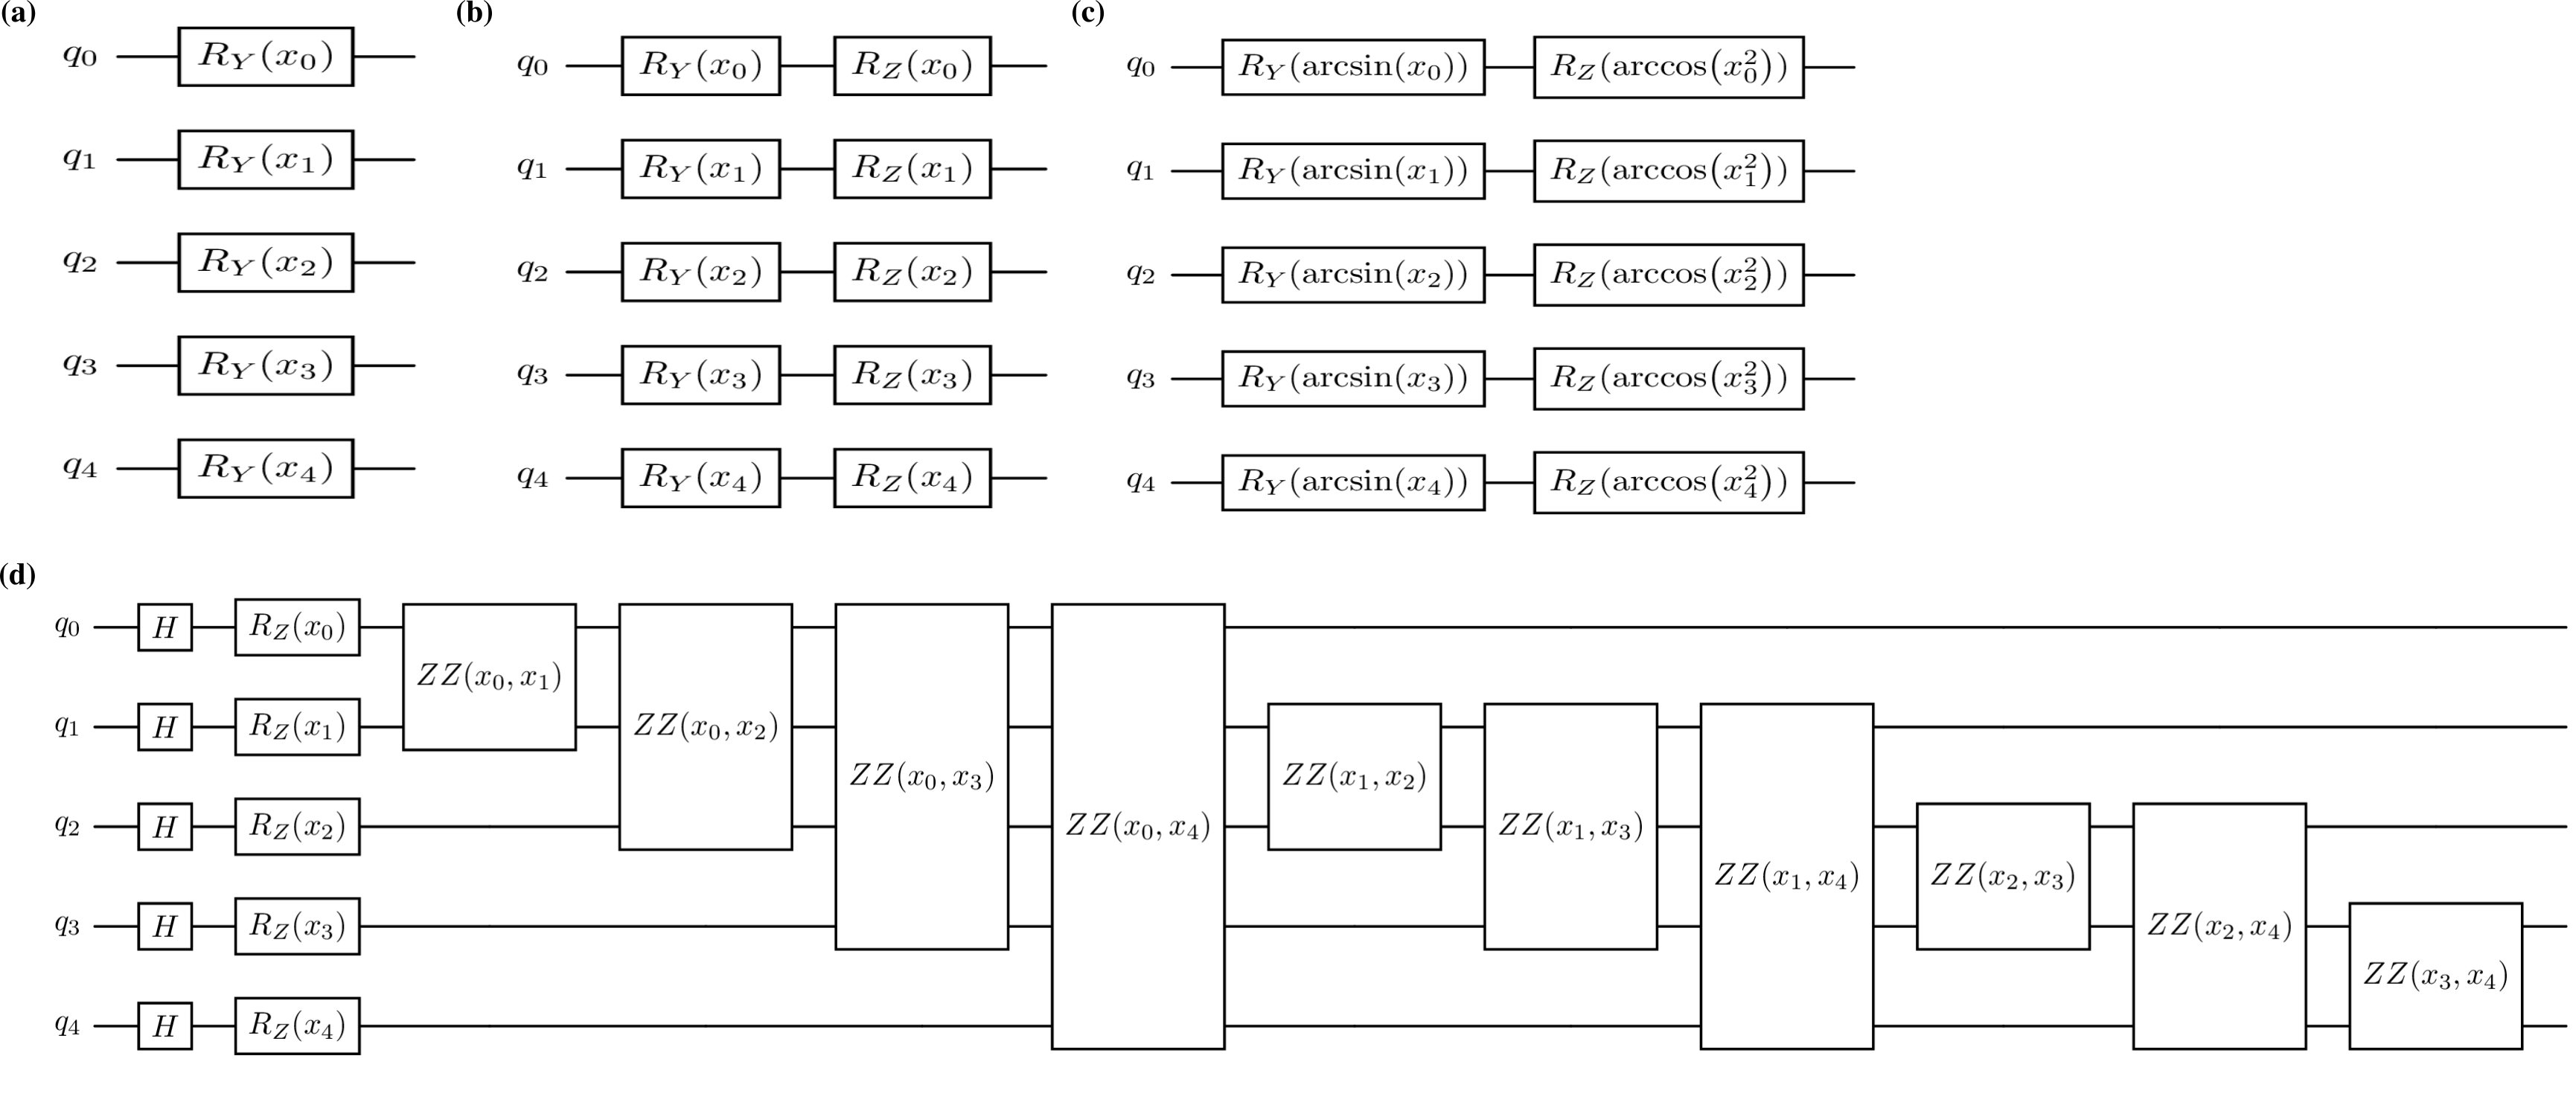
\includegraphics[width=\textwidth]{../images/encoders/quantikz/combined.png}
	\caption{Five qubit examples of the (a) single angle (A1), (b) double angle (A2), (c) Mitarai (M), and (d) Instantaneous Quantum Polynomial (IQP) encoders used in this study.}
	\label{fig:encoders}
\end{figure}

When $l=2$, more complex circuits can be generated, like in Ref. \citep{suzuki_predicting_2020}, where we choose the entanglement gates, $E_{\text{ent}}^{1}$ and $E_{\text{ent}}^{2}$, to be equivalent and the encoding layer takes the following form, $U_{\Phi(x)} =  E_{\text{ent}} U_{\phi_{2}(\mathbf{x})} E_{\text{ent}} U_{\phi_{1}(\mathbf{x})}$.
Additionally, we exclude IQP encoding when $l=2$ due to the increased computational costs associated with the circuit depth when compared to the expanded models based on A1, A2, and M encoding.
Therefore, when we exclude IQP, there are five unique combinations of $U_{\phi_{1}(\mathbf{x})}$ and $U_{\phi_{2}(\mathbf{x})}$ (M-M, A1-A1, A2-A2, M-A1, and M-A2) and two different entanglement layer options (CNOT and CZ) for a total of 10 encoding circuits with $l=2$.
The common notation for these circuits is $U_{\phi_{1}(\mathbf{x})}-U_{\phi_{2}(\mathbf{x})}-E_{\text{ent}}$ where two example encoding circuits are M--M--CNOT and M--A1--CNOT.
The 14 encoding circuits used throughout this study are shown in Table \ref{tab:encoders}, where the first column shows the label, second column the first unitary ($U_{\phi_{1}(\mathbf{x})}$), third column the second unitary ($U_{\phi_{2}(\mathbf{x})}$), and last column the entanglement gates ($E_{\text{ent}}$).

\begin{table}[htbp]
	\centering
	\begin{tabular}{|c|c|c|c|}
		\hline
		\textbf{Name} & $U_{\phi_{1}(\mathbf{x})}$ & $U_{\phi_{2}(\mathbf{x})}$ & $E_{\text{ent}}$  \\
		\hline
		\hline
		A1 & $U_{\text{A1}}$ & --- & --- \\
		\hline
		A2 & $U_{\text{A2}}$ & --- & --- \\
		\hline		
		M & $U_{\text{M}}$ & --- & --- \\
		\hline
		IQP & $U_{\text{IQP}}$ & --- & --- \\
		\hline
		A1--A1--CNOT & $U_{\text{A1}}$ & $U_{\text{A1}}$ & $E_{\text{CNOT}}$ \\
		\hline
		 A2--A2--CNOT & $U_{\text{A2}}$ & $U_{\text{A2}}$ & $E_{\text{CNOT}}$ \\
		\hline
		M--M--CNOT & $U_{\text{M}}$ & $U_{\text{M}}$ & $E_{\text{CNOT}}$ \\
		\hline
		M--A1--CNOT & $U_{\text{M}}$ & $U_{\text{A1}}$ & $E_{\text{CNOT}}$ \\
		\hline		
		M--A2--CNOT & $U_{\text{M}}$ & $U_{\text{A2}}$ & $E_{\text{CNOT}}$ \\
		\hline				
		A1--A1--CZ & $U_{\text{A1}}$ & $U_{\text{A1}}$ & $E_{\text{CZ}}$ \\
		\hline
		A2--A2--CZ& $U_{\text{A2}}$ & $U_{\text{A2}}$ & $E_{\text{CZ}}$ \\
		\hline
		M--M--CZ & $U_{\text{M}}$ & $U_{\text{M}}$ & $E_{\text{CZ}}$ \\
		\hline
		M--A1--CZ & $U_{\text{M}}$ & $U_{\text{A1}}$ & $E_{\text{CZ}}$ \\
		\hline		
		M--A2--CZ & $U_{\text{M}}$ & $U_{\text{A2}}$ & $E_{\text{CZ}}$ \\
		\hline						
	\end{tabular}
	\caption{The 14 encoding layers used in this study where the first column shows the encoding circuit name, the second column the unitary for $l=1$, the third column the unitary for $l=2$, and the last column the corresponding entanglement gates.}
	\label{tab:encoders}
\end{table}

The next layer in a PQC which follows the encoding layer, is the variational layer.
The variational layers introduce trainable parameters, that can be optimized using classical compute resources, into the quantum circuit and provide flexibility to the QML models.
These layers have a general form, defined as,
\begin{equation}
	U(\bm{\theta}) = \prod_{v} U_{v}(\bm{\theta}_{v}), % E_{\text{ent}}^{v}
	\label{eq:general_variational}
\end{equation}
where $\bm{\theta}$ denote the variational parameters, $v$ denote the number of times that the layer is repeated within the circuit, and all entanglement gates are implicitly included in $U_{v}(\bm{\theta}_{v})$.
In our study, we examine 12 variational circuits, found in \cite{sim_expressibility_2019}, as shown in Fig. \ref{fig:ansatz}.
The unique names of the 12 variational circuits are as follows: Modified-Pauli-CRZ (Fig. \ref{fig:ansatz}\textbf{(a)}) , Modified-Pauli-CRX (Fig. \ref{fig:ansatz}\textbf{(b)}), Efficient-CRZ (Fig. \ref{fig:ansatz}\textbf{(c)}), Efficient-CRX (Fig. \ref{fig:ansatz}\textbf{(d)}),, HWE-CNOT (Fig. \ref{fig:ansatz}\textbf{(e)}), HWE-CZ (Fig. \ref{fig:ansatz}\textbf{(f)}), ESU2 (Fig. \ref{fig:ansatz}\textbf{(g)}), Full-Pauli-CRZ (Fig. \ref{fig:ansatz}\textbf{(h)}), Full-Pauli-CRX (Fig. \ref{fig:ansatz}\textbf{(i)}), Hadamard (Fig. \ref{fig:ansatz}\textbf{(j)}), Full-CRZ (Fig. \ref{fig:ansatz}\textbf{(k)}), and Full-CRX (Fig. \ref{fig:ansatz}\textbf{(l)}).

\begin{figure}[H]
	\centering
	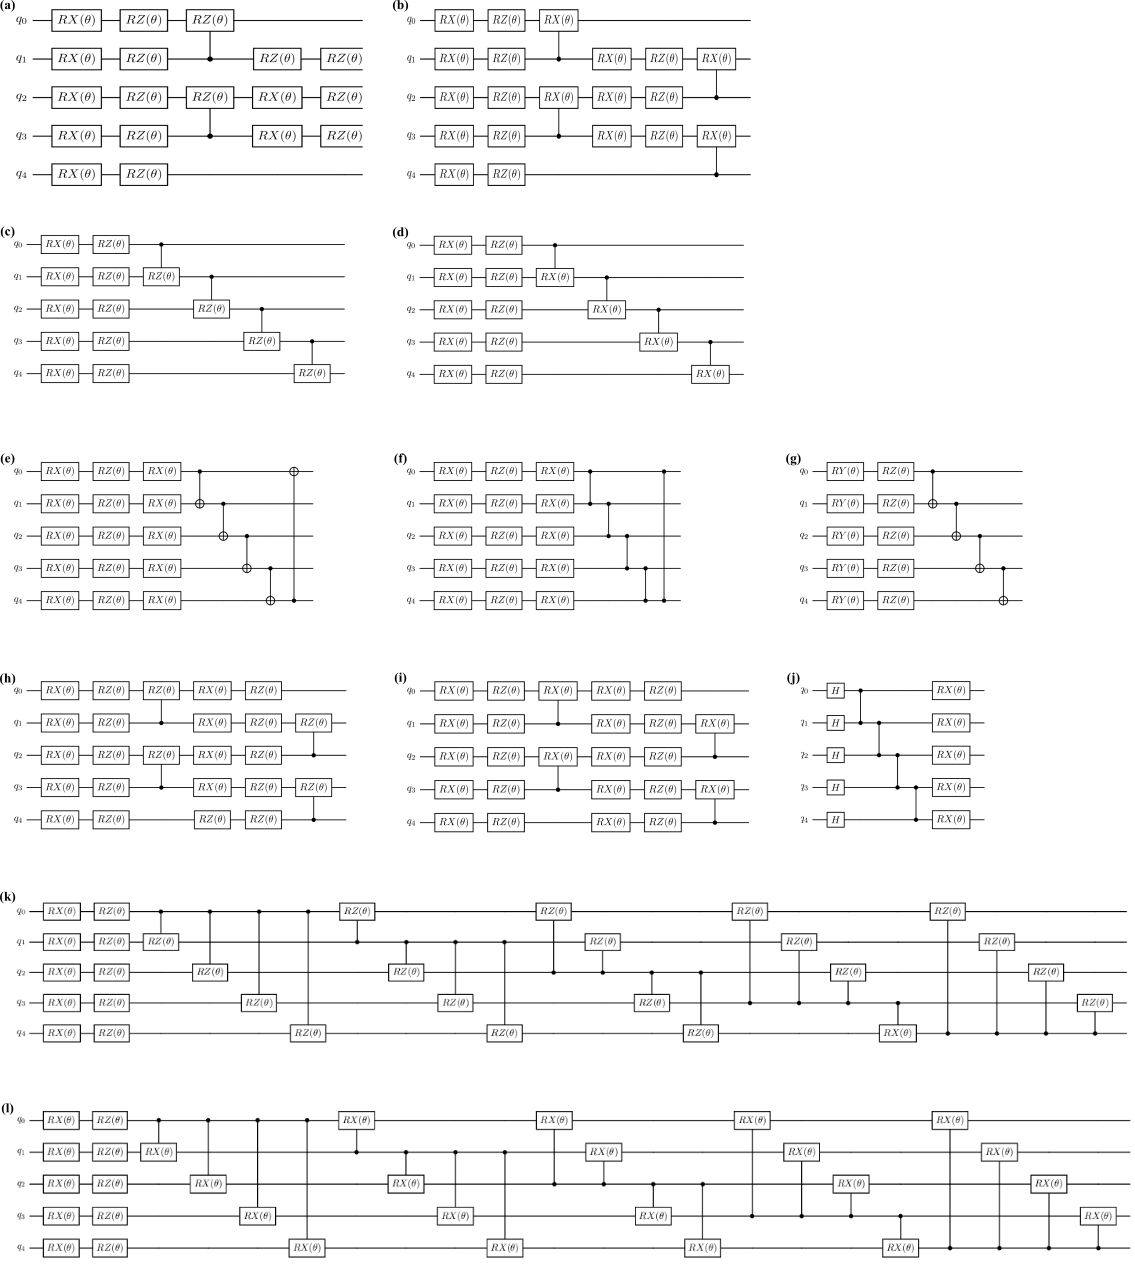
\includegraphics[width=\textwidth]{../images/ansatz/quantikz/combined.png}
	\caption{The 12 variational circuits include (a) Modified-Pauli-CRZ, (b) Modified-Pauli-CRX, (c) Efficient-CRZ, (d) Efficient-CRX, (e) HWE-CNOT, (f) HWE-CZ, (g) ESU2, (h) Full-Pauli-CRZ, (i) Full-Pauli-CRX, (j) Hadamard, (k) Full-CRZ, and (l)Full-CRX}
	\label{fig:ansatz}
\end{figure}


To introduce more model parameters and increase the expressibility and nonlinearity of the PQCs, two expansion strategies can be explored.
The first we denoted as the number of ansatz layers (AL), where $v$ can be increased to introduce more unique trainable parameters into the PQC.
The second expansion strategy builds on the work of P\'{e}rez-Salinas \textit{et al.} that showed data re-uploading in PQCs is equivalent to the Universal Approximation Theorem for artificial neural networks.\cite{perez-salinas_data_2020}
This is achieved by combining Eqs. \ref{eq:general_encoding} and \ref{eq:general_variational} into a general circuit,

\begin{equation}
	\ket{\Psi} = U(\bm{\theta}) U_{\Phi(\mathbf{x})}\ket{0}^{\otimes n} = \prod_{k}
	\left( \prod_{v} U_{v}(\bm{\theta}_{v}) \prod_{l} E_{\text{ent}}^{l} U_{\phi_{l}(\mathbf{x})} \right)  \ket{0}^{\otimes n},
\end{equation}
where $k$ denotes the re-upload depth (RUD) of the circuit.

The last component of a PQC is the measurement, which is required to recover the predicted target values, $\hat{y}_{i}$, of the machine learning model that is used to update the model parameters.
This is performed by measuring the quantum state, $\ket{\Psi}$, using the Pauli Z operator on the first qubit denoted as,
\begin{equation}
	\hat{y}_{i} = \bra{\Psi}Z_{0}\ket{\Psi}_{i},
	\label{eq:y_pred}
\end{equation}
and passing the set of predicted target values, $\bm{\hat{y}} = (\hat{y}_{1}, \ldots, \hat{y}_{N}) \in \mathbb{R}^{N}$, where $N$ is the number of samples, to the loss function, $\mathcal{L}(\bm{y}, \bm{\hat y})$, where $y_{i}$ belongs to the set of true target values $\bm{y} = (y_{1}, \ldots, y_{N}) \in \mathbb{R}^{N}$.
While $\mathcal{L}$ can be any loss function relevant for regression-based ML tasks, we choose to mean square error to be the loss function,
\begin{equation}
	\mathcal{L}(\bm{y}, \bm{\hat y}) = \frac{1}{N} \sum_{i=1}^{N} (y_{i} - \hat{y}_{i})^{2}.
	\label{eq:isthisloss}
\end{equation}


\section{Implementation}
To explore the large combination of PQCs previously mentioned, we introduce \textit{qregress} (Fig. \ref{fig:overview_project}), a modular Python package based on PennyLane\cite{bergholm_pennylane_2022} and Qiskit\cite{javadi-abhari_quantum_2024}.
The portion of the code based on PennyLane is capable of performing state-vector simulation using Qulacs\cite{suzuki_qulacs_2021}, noisy simulation using \textit{qiskit-aer} with the \textit{FakeQuebec} backend, along with access to real devices accessible on the IBM Quantum Platform using the PennyLane-Qiskit plugin.
Additionally, to train and test regression models that require many circuit executions, we ported our PennyLane code to Qiskit so that the Qiskit Batch Execution mode could be utilized.
This was a vital step for running on \textit{ibm\_quebec} since Qiskit Sessions, as implemented in the PennyLane-Qiskit plugin, are too cumbersome to train PQCs as $N$, the number of training samples, increases.
In practice, all state-vector simulations were performed using PennyLane, while all calculations using \textit{FakeQuebec} and \textit{ibm\_quebec}  are run using Qiskit.
All state-vector simulations with 5 qubits were optimized using 1000 iterations, while 16 qubits were initially run using 250 iterations.
State-vector simulations were also optimized using the Simultaneous Perturbation Stochastic Approximation method (SPSA), as implemented in PennyLane since we found that SPSA requires fewer steps to optimize when compared to other optimizers for state-vector simulation. 
For the experiments ran using \textit{FakeQuebec} and  \textit{ibm\_quebec}, we utilized the Constrained Optimization By Linear Approximation (COBYLA) optimizer, as implemented in SciPy\cite{virtanen_scipy_2020}.
For all models, features ($\mathbf{x}$) and target values ($\mathbf{y}$) were scaled using the MinMaxScaler, as implemented in Scikit-learn\cite{pedregosa_scikit-learn_2011}, such that all features and target values are $\mathbb{R}\in [ -1,1 ]$.



\begin{figure}[H]
	\centering
	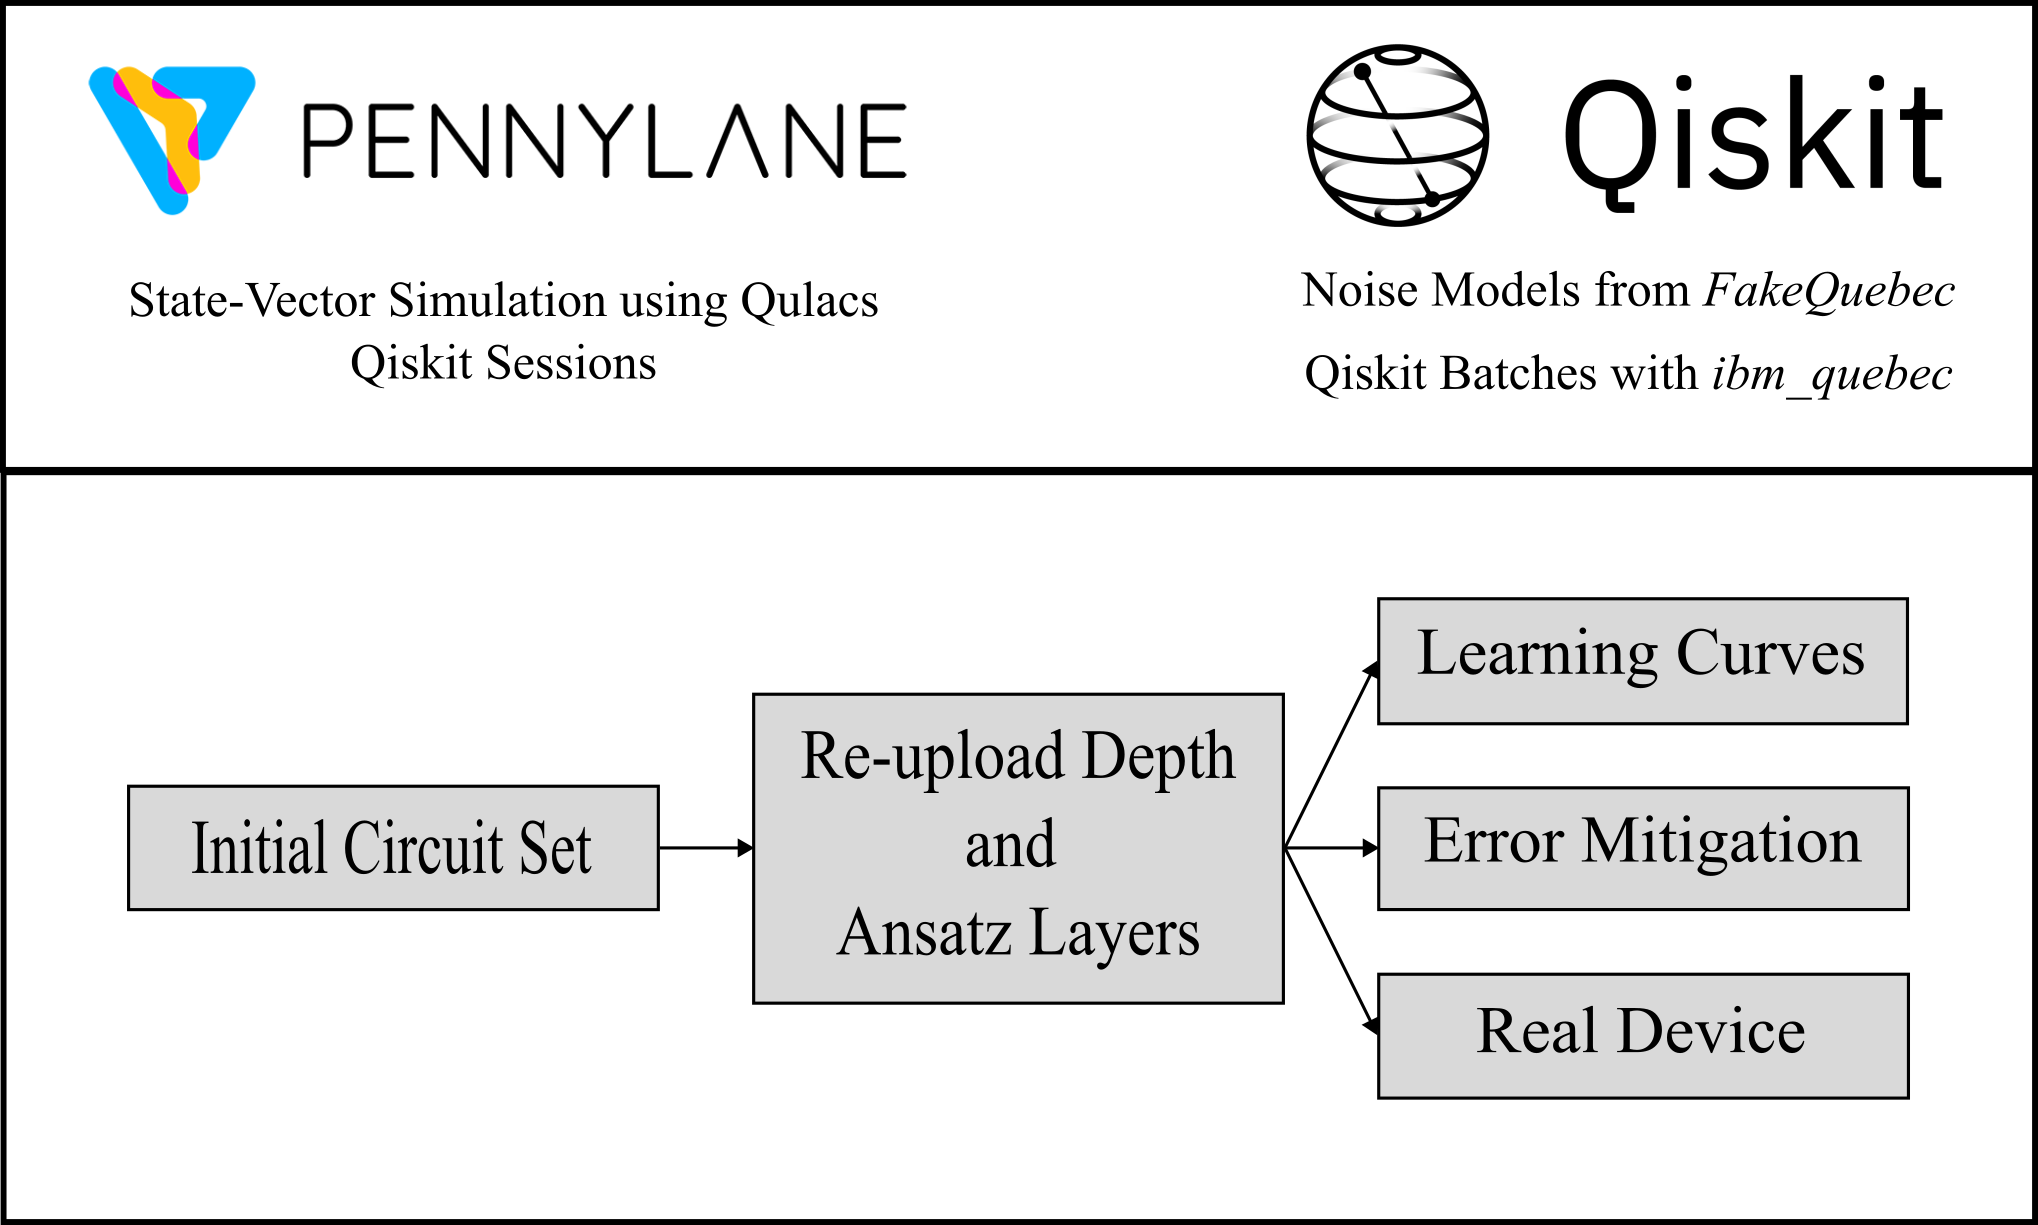
\includegraphics[width=\linewidth]{../images/manuscript_figures/overview.png}
	\caption{REMAKE to include cool code pic. Make this figure highlight the modularity of \textit{qregress}}
	\label{fig:overview_project}
\end{figure}







\section{Datasets}\label{subsection:datasets}

The first quantum chemistry dataset we explore is BSE49, which contains bond separation energies (BSEs), for homolytic bond cleavage of covalently bonded molecules, such as \ce{A-B -> A^{.} + B^{.}}.\cite{prasad_bse49_2021}
This dataset consists of 49 unique A-B type bonds with 4394 datapoints, 1951 of which are existing structures, while the remaining 2443 are hypothetical structures. 
BSE49 provides highly accurate BSEs, calculated using the  (RO)CBS-QB3\cite{wood_restricted-open-shell_2006,montgomery_complete_1999,montgomery_complete_2000} composite quantum chemistry method, that is useful for benchmarking ML-based applications.


An important aspect of ML in chemistry is the choice of molecular representation, or how the molecule is represented in the machine learning models.\cite{jones_molecular_2023}
In general, molecular representations can be partitioned into three groups, graph-, topology-, and physics-based representations, all of which were explored to provide a comprehensive overview of how they perform using classical models as a baseline.
During the preprocessing stage, before converting the XYZ coordinates into our molecular representation of choice, the set of hypothetical structures was reduced to 2436 molecules due to issues with valency exceptions when converting XYZ coordinates into RDKit mol objects.
Using RDKit\cite{noauthor_rdkit_nodate} we examined three commonly applied graph-based molecular preresentations, Molecular ACCess Systems (MACCS)\cite{durant_reoptimization_2002}, Morgan or extended-connectivity fingerprints \cite{morgan_generation_1965,rogers_extended-connectivity_2010}, and RDKit fingerprints.
All three of these methods use traversals of the molecular graphs to encode various structural details into bit vectors.
Lastly, we explore both topology- and physics-based molecular representations, both of which encode the three-dimensional structure of molecules in various, unique ways.
Persistent images (PIs) are a topology-based fingerprint that uses persistence homology to encode topological information of three-dimensional molecular structures into fixed-dimension images.\cite{adams_persistence_2017,townsend_representation_2020,schiff_augmenting_2022} 
We use the implementation from Townsend \textit{et al.}\cite{townsend_representation_2020}, which uses the Ripser Python package to generate PIs.\cite{tralie_ripserpy_2018}
Lastly, we explore two physics-based representations, Coulomb matrices (CMs) \cite{rupp_fast_2012} and smooth overlap of atomic positions (SOAPs), that were generated using DScribe.\cite{de_comparing_2016}
Both methods encode physical information regarding the atomic environments of each molecule, where CMs encode the Coulomb repulsion between atoms using nuclear charges, while SOAPs encode the similarities between atomic neighborhoods using kernels.
Due to the computational cost associated with computing the regularized entropy match (REMatch) kernel over the set of 2436 molecules with the SOAPs representation, we excluded SOAPs from the overall discussion.
For each of the molecular representations, we analyzed two different methods for representing the components of the BSE reaction.
The first represents the feature vector as the products subtracted from the reactants, denoted as \textit{sub} (e.g., $\mathbf{X}_{\mathit{sub}} = (\mathbf{X}_{\text{A}^{.}} + \mathbf{X}_{\text{B}^{.}}) - \mathbf{X}_{\text{A-B}}$), similar to the method used in Ref. \cite{garcia-andrade_barrier_2023}, and the second represents the feature vector using only the reactant (A-B), denoted as \textit{AB} (e.g., $\mathbf{X}_{\mathit{AB}} =  \mathbf{X}_{\text{A-B}}$).


Using this set of molecular representations, we also examine a diverse set of classical regression models to help choose the optimal representation for our diverse set of PQCs.
The classical models we analyze include ridge, lasso, elastic net, \textit{k}-nearest-neighbors, random forest, gradient boosting, support vector machines, kernel ridge, and Gaussian process regression as implemented in sckit-learn.\cite{pedregosa_scikit-learn_2011}
As highlighted in Fig. \ref{fig:classical_molrepfig}, we found that the best molecular representation across all models tested was Morgan fingerprints using the \textit{sub} formulation, which we use for all experiments using the PQCs.
Additionally, one challenge of applying classical molecular representations for ML tasks using PQCs is reducing the set of features, often containing hundreds or thousands of features per sample, to the number of qubits used on the quantum device.
For example, at the onset of this project, the standard number of qubits on the IBM quantum devices was 5 or 16 qubits, which requires reducing the initial set of 2048 features per sample for Morgan fingerprints down to 5 or 16 features.
To perform this reduction, we explored two different methods, SHapley Additive ExPlanation analysis (SHAP)\cite{lundberg_unified_2017}, which uses cooperative game theory to determine feature importance, and principal component analysis (PCA), which is a dimensionality reduction technique that captures the direction a datasets variance, as implemented in scikit-learn.\cite{pedregosa_scikit-learn_2011}
In Figs. \ref{fig:BSE_classical_features_R2} and \ref{fig:BSE_bse_classical_features_MAE}, we compare the two reduction techniques, for both 5 and 16 features, with the initial model containing 2048 features.
The initial model has mean absolute errors (MAE) of 1.91 and 4.98 kcal/mol and R$^{2}$s of 0.99 and 0.91 for the training and test set, respectively.
Using SHAP, we found that the model containing 5 features has an MAE of 16.08 kcal/mol and an R$^{2}$ of 0.39 for the training set, while the test set has an MAE of 15.86 kcal/mol and an R$^{2}$ of 0.42.
For the model with 16 features, we observe improvements in both the training and test sets, with MAEs of 10.48 and 11.08 kcal/mol and R$^{2}$ values of 0.69 and 0.68, respectively.
For the models using 5 and 16 features reduced through PCA, the training sets yield MAEs of 4.09 and 3.23 kcal/mol, while the test sets have MAEs of 10.17 and 8.40 kcal/mol, respectively.
The R$^{2}$s also show slight improvement over the feature reductions using SHAP, where the R$^{2}$s using 5 features are 0.95 and 0.69 for the training and test set, respectively, and the model using 16 features has R$^{2}$s of 0.97 and 0.78 for the training and test set, respectively.
Overall, the models using SHAP to reduce the feature set offer models with less overfitting, while sacrificing accuracy, when compared to the models reduced using PCA, which offer more accurate models that are more overfit. 
Based on these insights, for the experiments using PQCs, all BSE49 data is reduced to 5 or 16 qubits using PCA applied on Morgan fingerprint using the \textit{sub} formulation.

The second quantum chemistry dataset we analyze in this paper is generated using the data-driven coupled-cluster (DDCC) scheme of Townsend and Vogiatzis.\cite{townsend_data-driven_2019,jones_chapter_2023}
DDCC is an ML-based approach for accelerating the convergence of coupled-cluster singles and doubles (CCSD) calculations by predicting the $t_{2}$-amplitudes of the CCSD wave function (Eq. \ref{eq:cc_wfn}) with features generated using lower-level methods, such as Hartree-Fock (HF) and M{\o}ller-Plesset second-order perturbation theory (MP2), that are used to initialize CCSD calculations.
Herein, we provide a brief overview of the equations required to understand the DDCC method, starting with the coupled-cluster wave function, which takes the general form,
\begin{equation}
	\ket{\Psi_{\text{CC}}} = \exp(\hat{T}) \ket{\Psi_{0}}
	\label{eq:cc_wfn}
\end{equation}
where $\hat{T}$ is the cluster operator and $\ket{\Psi_{0}}$ is the reference (Hartree-Fock) wave function.
In CCSD, the $\hat{T}$ operator is truncated to only include single ($\hat{T}_{1}$) and double ($\hat{T}_{2}$) excitations.
After solving the coupled-cluster equations, the CCSD correlation energy can be formulated as,
\begin{equation}
	E^{\text{CCSD}}_{\text{corr}} = \sum_{\substack{a<b \\ i<j}} \mel{ij}{}{ab} t^{ab}_{ij} + \sum_{\substack{a<b \\ i<j}} \mel{ij}{}{ab} t^{a}_{i} t^{b}_{j}
	\label{eq:cc_corr}
\end{equation}
where $i$ and $j$ denote occupied orbitals, $a$ and $b$ denote virtual orbitals, $t^{ab}_{ij}$ correspond to two-electron excitation amplitudes ($t_{2}$-amplitudes), $t^{a}_{i}$ and $t^{b}_{j}$ correspond to one-electron excitation amplitudes ($t_{1}$-amplitudes), and $\mel{ij}{}{ab}$ are two-electron integrals.
The objective of the DDCC method is to learn the CCSD $t_{2}$-amplitudes using features generated using HF and MP2, since the CCSD $t_{2}$-amplitudes are initialized using MP2 $t_{2}$-amplitudes, defined as,
\begin{equation}
	t^{ab}_{ij(\text{MP2})} = \frac{\mel{ij}{}{ab}}{\varepsilon_{i}+\varepsilon_{j}-\varepsilon_{a}-\varepsilon_{b}}
	\label{eq:MP2_t2}
\end{equation}
where $\varepsilon_{i}$ and $\varepsilon_{j}$ denote the orbital energies of the occupied orbitals $i$ and $j$, while the virtual orbitals $a$ and $b$ are denoted by $\varepsilon_{a}$ and $\varepsilon_{b}$.
Due to this important relationship, MP2 $t_{2}$-amplitudes are included in the DDCC feature set, along with the numerator ($\mel{ij}{}{ab}$), denominator ($\varepsilon_{i}+\varepsilon_{j}-\varepsilon_{a}-\varepsilon_{b}$), a binary feature to denote whether the excitation goes to the same virtual orbital, and the orbital energies ($\varepsilon_{i},\varepsilon_{j},\varepsilon_{a},\varepsilon_{b}$).
Additionally, the feature set includes terms related to the individual contributions to the orbital energies, such as the one-electron Hamiltonian ($h$), Coulomb matrix ($J$), exchange matrix $K$, and Coulomb and exchange integrals ($J^{i}_{a}, J^{j}_{b}, K^{a}_{i}, K^{b}_{j}$).
In total, there are 30 features for each CCSD $t_{2}$-amplitude due to the addition of features that denote the sign and magnitude of the MP2 $t_{2}$-amplitudes.

Using the DDCC method, we generate a dataset consisting of 199 water molecules obtained from the study of Townsend and Vogiatzis using the STO-3G basis set\cite{hehre_selfconsistent_1970}  with the frozen core approximation.
All HF, MP2, and CCSD data was generated using Psi4\cite{parrish_psi4_2017} and Psi4Numpy\cite{smith_psi4numpy_2018}.
We will also note that despite using a minimal basis set, this is a data-intensive quantum chemistry application for PQCs since for each molecule there are $(N_{occ})^{2}(N_{virt})^{2}$ $t_{2}$-amplitudes, where $N_{occ}$ denotes the number of occupied orbitals and $N_{virt}$ denotes the number of virtual orbitals.
For the water confirmers with 4 occupied and 2 virtual orbitals, there are a total of 64 $t_{2}$-amplitudes per molecule.
Further details regarding the feature set and implementation can be found in Ref.  \cite{townsend_data-driven_2019}

Lastly, like the BSE49 dataset, the 30 DDCC features must be reduced to 5 or 16 features using either SHAP or PCA.
Unlike the BSE49 dataset, SHAP outperforms PCA due to the direct relationship between the feature set and target values.
Additionally, as highlighted in Fig. \ref{fig:DDCC_feature_set}, when the feature set is reduced to 5 or 16 features, both models have train and test R$^{2}$s of 1.00.
Due to the computational costs of simulating state-vector models on a broad set of PQCs, we will only perform our DDCC models with 5 features, which includes the two-electron integrals ($\mel{ij}{}{ab}$), MP2 $t_{2}$-amplitudes ($t^{ab}_{ij(\text{MP2})}$), the magnitude of the MP2 $t_{2}$-amplitudes, the difference in orbital energies ($\varepsilon_{i}+\varepsilon_{j}-\varepsilon_{a}-\varepsilon_{b}$), and the binary feature denoting whether two-electrons are promoted to the same virtual orbital ($a=b$).



\begin{figure}[H]
	\centering
	\begin{subfigure}[b]{0.65\textwidth}
		\centering
		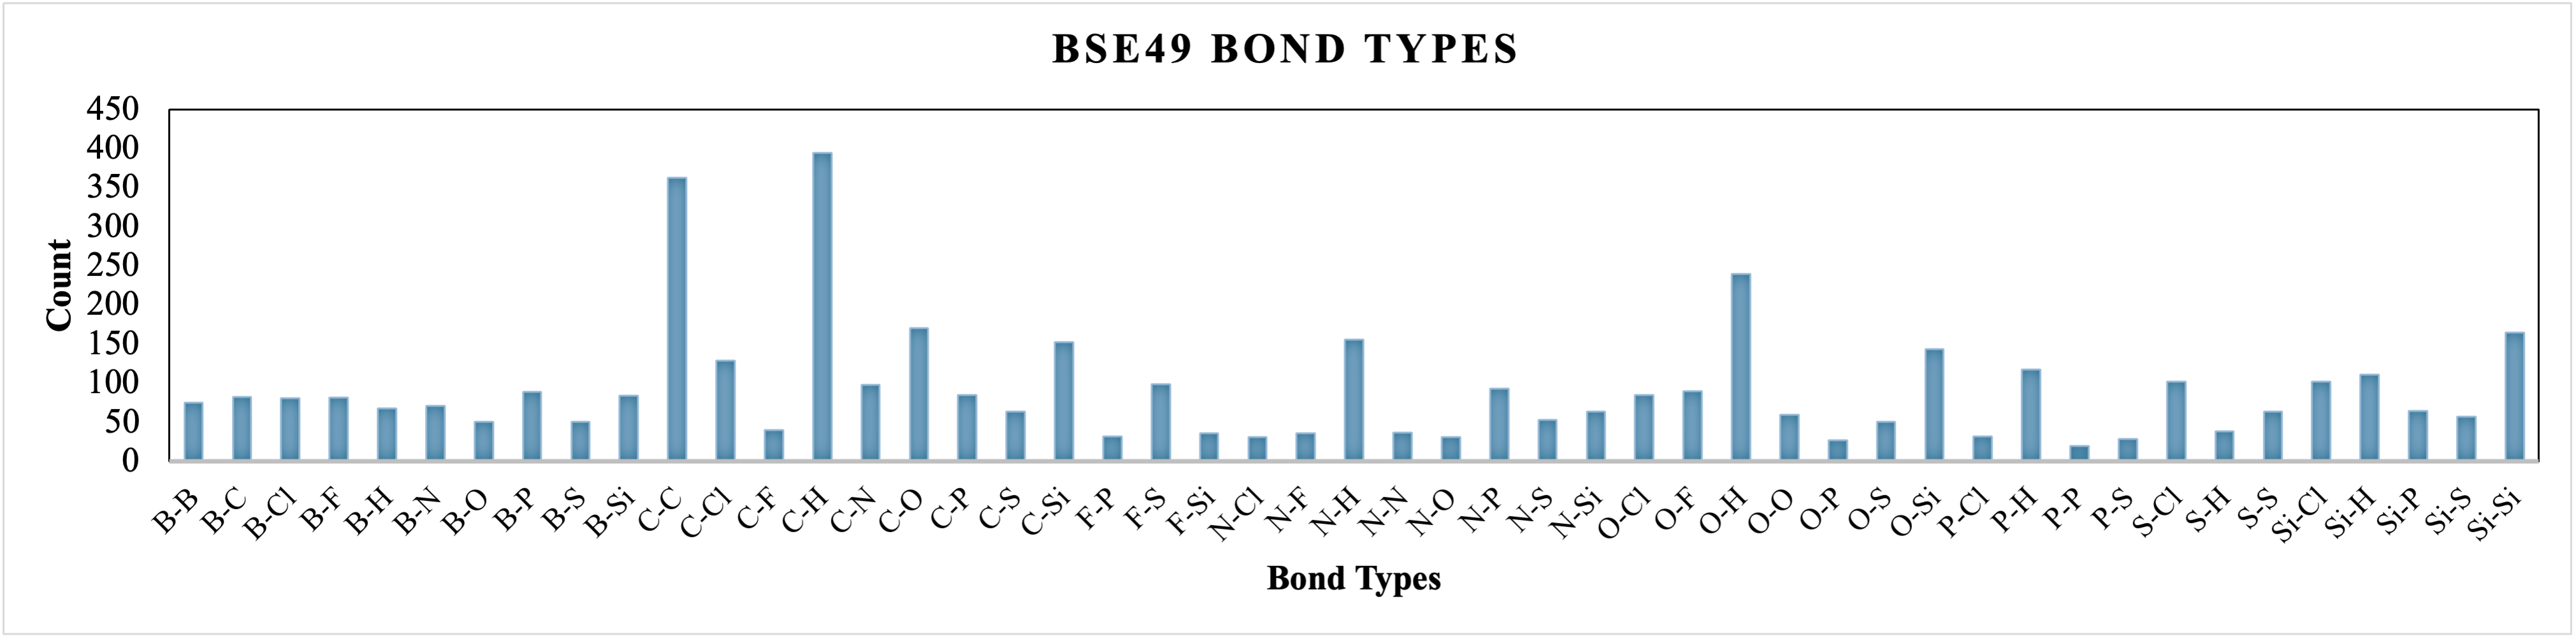
\includegraphics[width=\textwidth]{../images/BSE/bondtypes.png}
		\caption{}
		\label{fig:bondtypes}
	\end{subfigure}
	\hfill
	\begin{subfigure}[b]{0.3\textwidth}
		\centering
		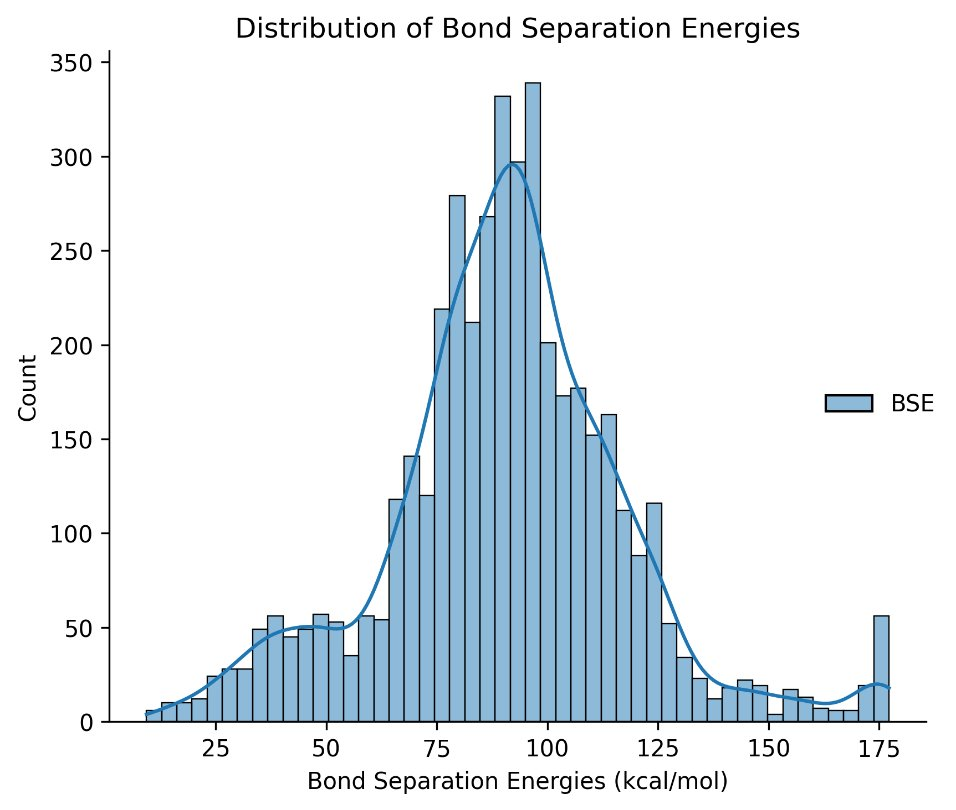
\includegraphics[width=\textwidth]{../images/BSE/BSE.jpg}
		\caption{}
		\label{fig:BSEdistr}
	\end{subfigure}
	\hfill
	\begin{subfigure}[b]{0.3\textwidth}
		\centering
		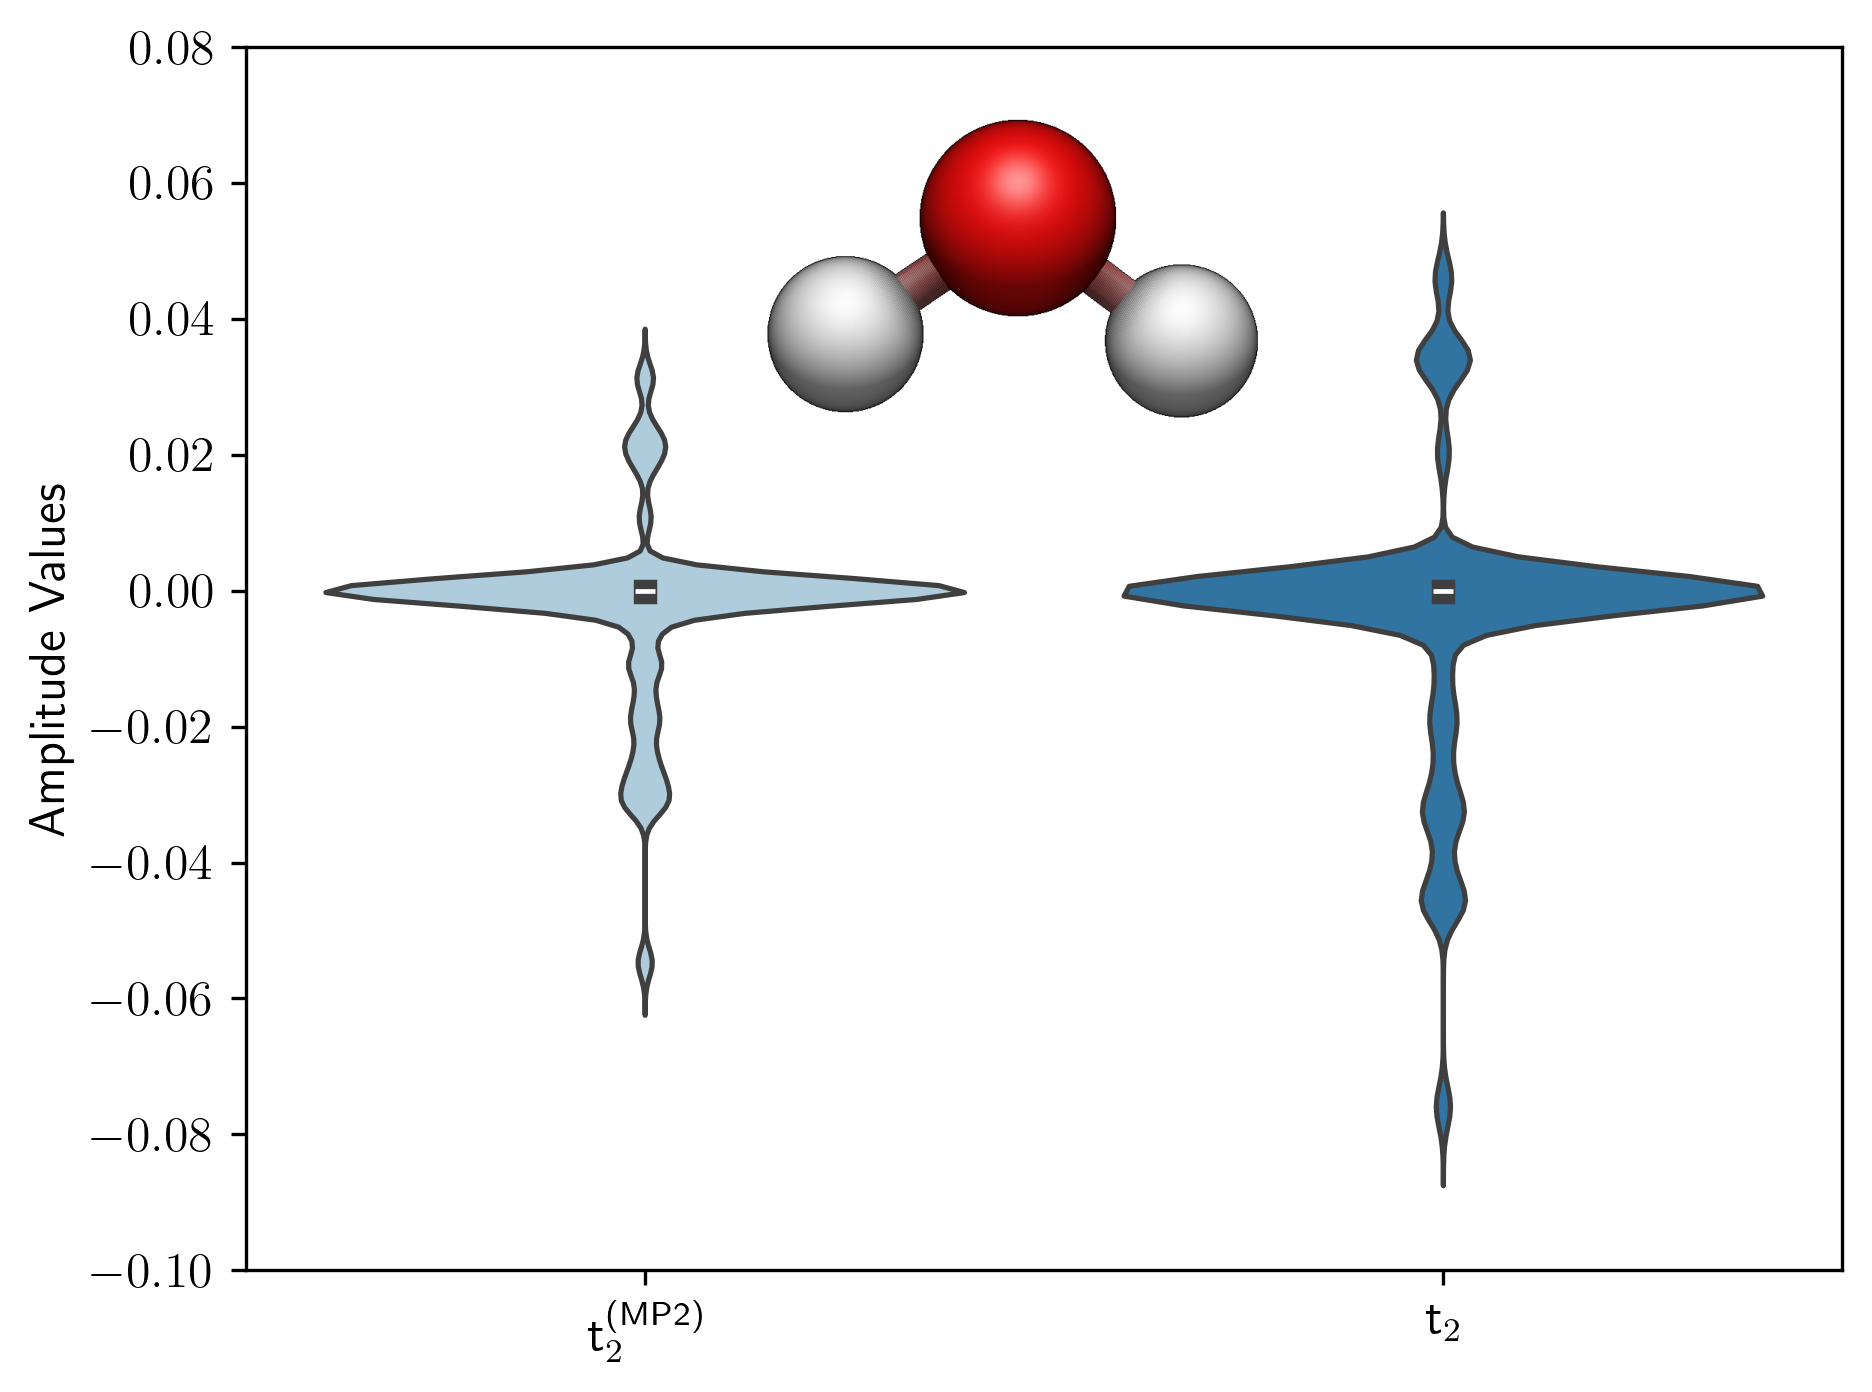
\includegraphics[width=\textwidth]{../images/manuscript_figures/waterddccdistribution.png}
		\caption{}
		\label{fig:waterddccdistribution}
	\end{subfigure}	
	\caption{REMAKE: Examples of the datasets explored in this study. For the BSE49 dataset the distributions of the (d) bond types and the (e) bond separation energies in kcal/mol. For the DDCC dataset distributions of the initial MP2 $t_{2}$-amplitudes and the optimized CCSD $t_{2}$-amplitudes are shown in (f).}
	\label{fig:bse_data}
\end{figure}





\section{Results and Discussion}
\label{section:results_and_discussion}
[introduction paragraph]
In this section, for both the DDCC and BSE49 datasets, we start our analysis by examining the performance of the initial set of 168 PQCs with re-upload depths of 1 ($k=1$) and the number ansatz layers set to 1 ($v=1$).
Using this data, we select the best encoder-ansatz pair and increase the re-upload depth and number of ansatz layers to 3 and 5 ($k,v \in {3,5}$) to determine how model performance is affected by circuit depth.
We then analyze how the best circuit from this set performs using a learning curve, where we hold the number of test points set to 20\% and vary the number of training points, to determine how PQCs behave with varying numbers of training data.
Lastly, we provide insights into how the best PQC model behaves on simulated and real IBM backends using \textit{FakeQuebec} and \textit{ibm{\_}quebec}.


Starting with the 5 qubits BSE49 data, Fig. \ref{fig:5BSE_heatplots} highlights the performance of the 168 PQCs using a heat plot of the coefficients of determination (R$^{2}$) of the training (left) and test sets (right).
The training set R$^2$ values range from a minimum of -1.4673 to a maximum of 0.1775, with a mean of -0.1865 and a standard deviation of 0.3433. 
For the test set, the R$^2$ values range from a minimum of -1.4774 to a maximum of 0.1974, with a mean of -0.1765 and a standard deviation of 0.3446.
General trends regarding the performance of the encoders (left) and ansatz (right) layers are highlighted in Fig. \ref{fig:5BSE_boxplots} using box plots.
On average, the best encoding layer is M-M-CNOT with a training and test R$^{2}$s of -0.0173 and -0.0157, respectively.
The best ansatz layer is Full-CRX with an average training  R$^{2}$ of 0.1054 and test R$^{2}$ of 0.1165.
Overall, for the BSE49 dataset using 5 qubits, the best encoder-ansatz pair is A1-A1-CNOT{\_}Full-CRX training set R$^{2}$ of 0.1775 and test set R$^{2}$ of 0.1974.
Despite A1-A1-CNOT{\_}Full-CRX being the best encoder-ansatz pair, for explorations of the circuit depth, we chose M-M-CZ{\_}HWE-CNOT, which offers similar performance training set R$^{2}$ of 0.1566 and test set R$^{2}$ of 0.1740 but has offered a more shallow circuit, which is more computationally efficient for state-vector simulations.

Following the 5 qubit models, we tested the BSE49 dataset on the set of 168 PQCs using 16 qubits.
Fig. \ref{fig:16BSE_heatplots} shows the performance in R$^{2}$ for the training (left) and test (right) sets, where the best encoder-ansatz pair is A1{\_}Efficient-CRZ with an R$^{2}$ of -0.0007 for the training set and -0.0050 for the test set.
Across the 168 PQCs, the training and test sets have a minimum R$^{2}$ -1.8104 and -1.7752, a mean of -0.4045 and -0.4022, a maximum of -0.0007 and -0.0004, and a standard deviation of 0.4161 and 0.4235, respectively.
Overall, as highlighted in Fig. \ref{fig:16BSE_boxplots} (left), the best encoder is IQP with a mean R$^{2}$ of -0.0942 for the training set and -0.0882 for the test set.
The best ansatz circuit (Fig. \ref{fig:16BSE_boxplots} right) is HWE-CNOT with a mean R$^{2}$ of -0.0148 and -0.0025 for the training and test set, respectively.
Due to the overall poorer performance and high computational expense of state-vector simulation using 16 qubits, we use only the best 5-qubit PQC, M-M-CZ{\_}HWE-CNOT, for the additional experiments with the BSE49 dataset.



\begin{figure}[H]
	\centering	
	\begin{subfigure}[b]{0.49\textwidth}
		\centering
		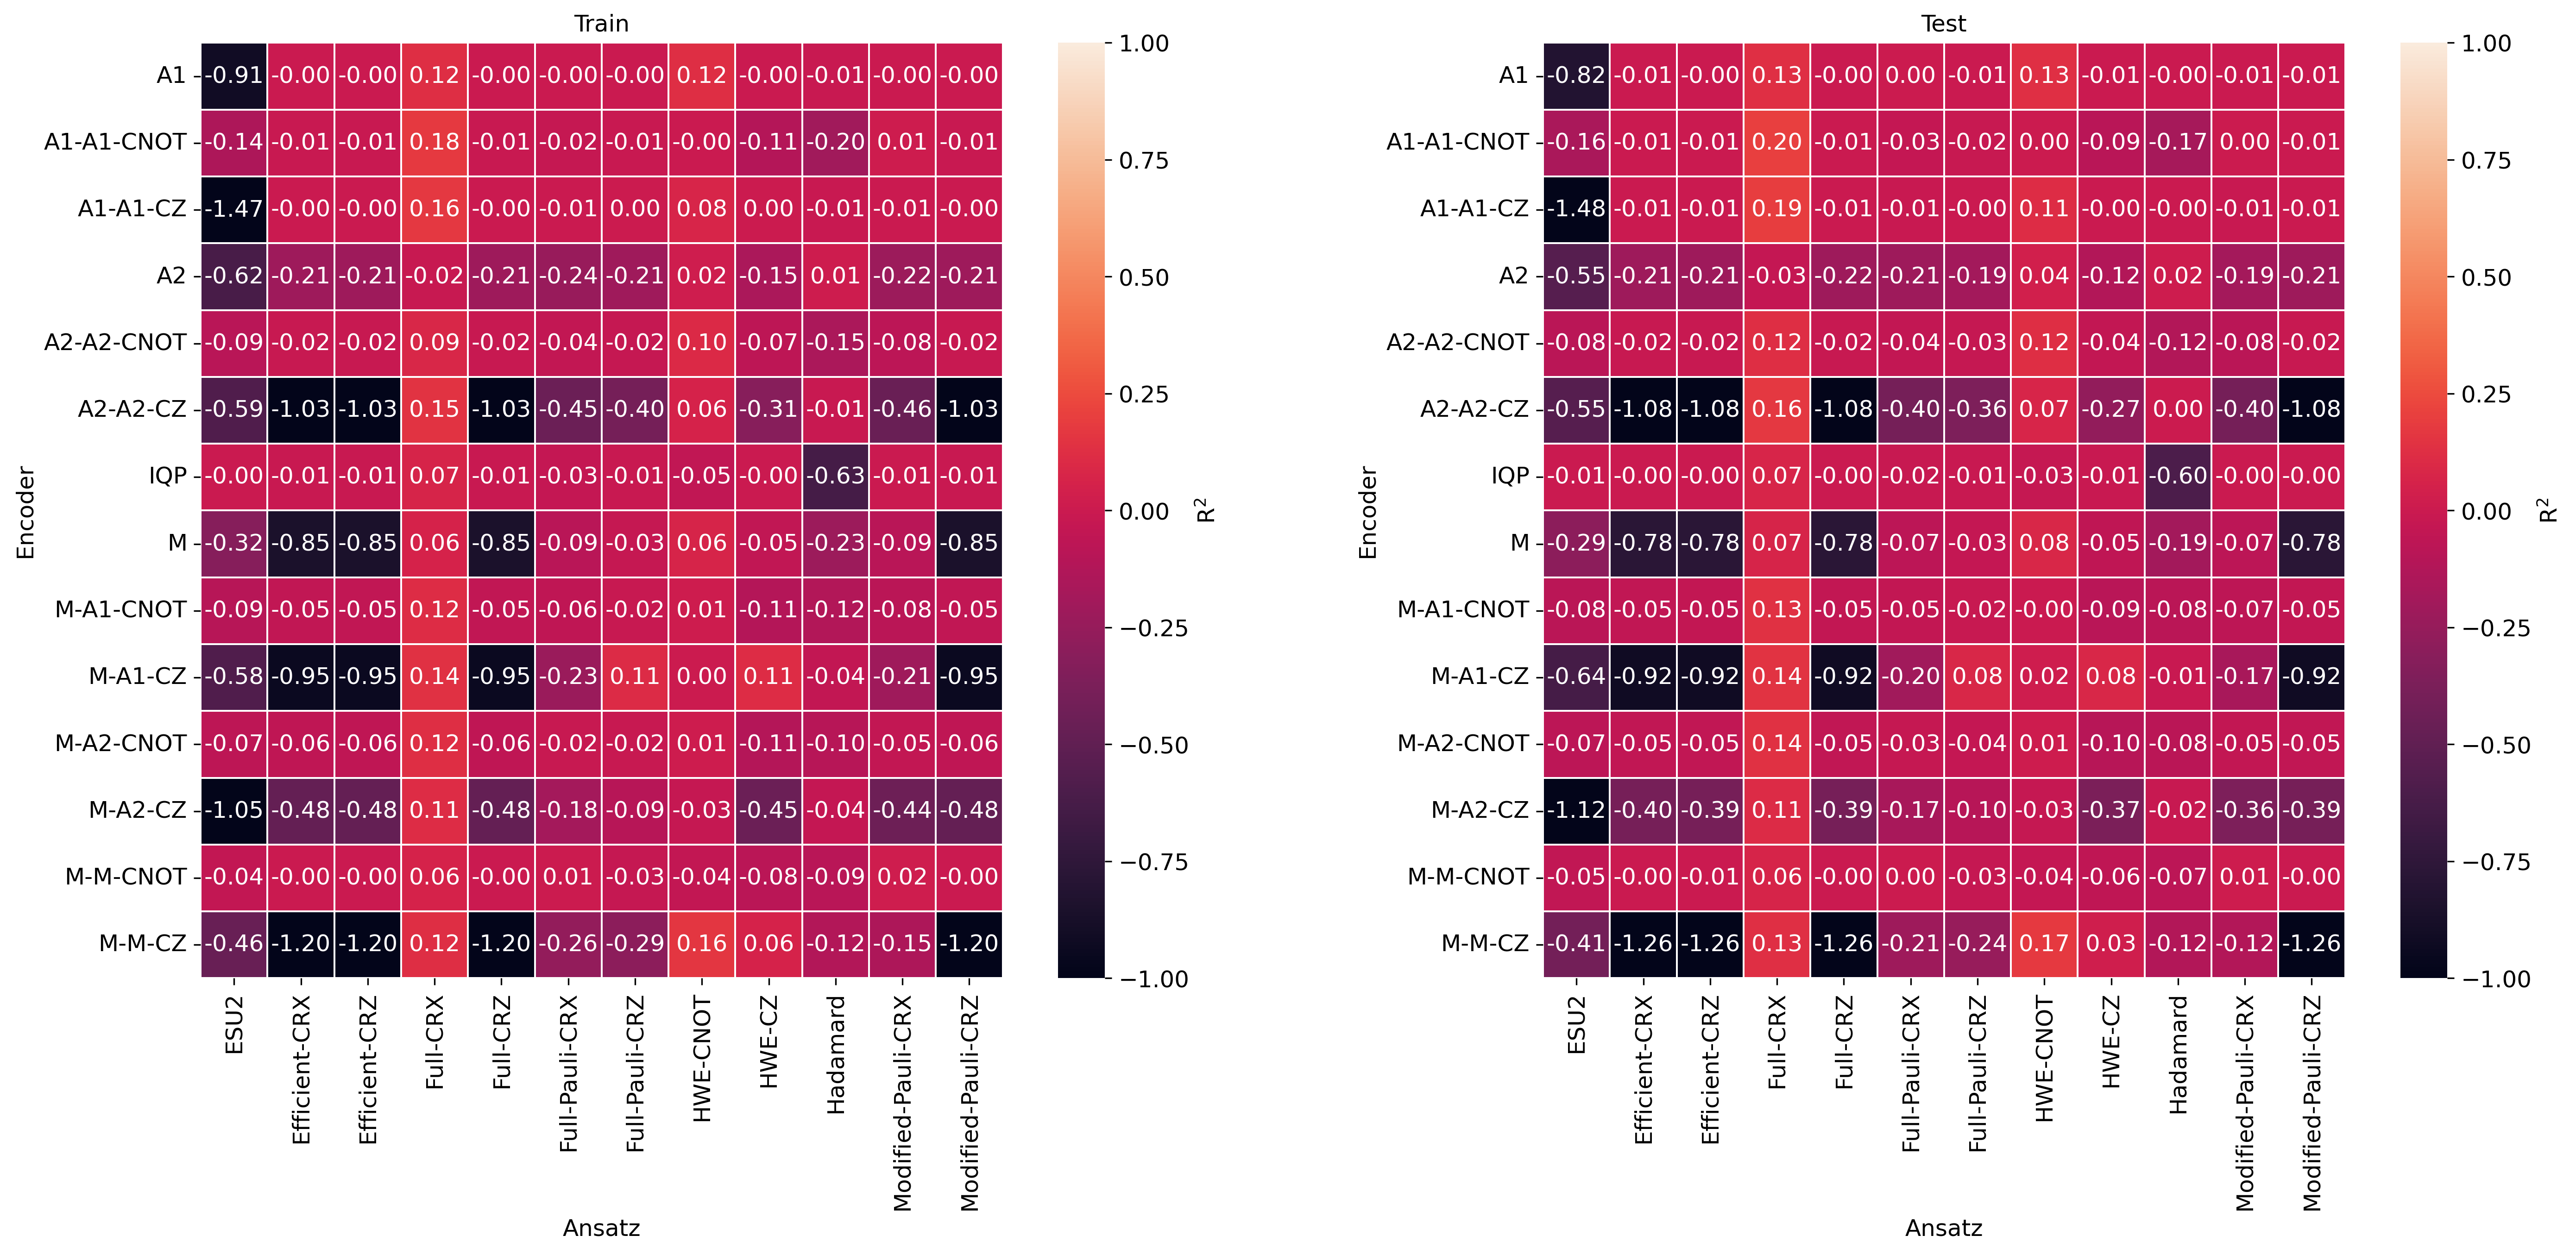
\includegraphics[width=\linewidth]{../images/BSE/fivequbit/BSE_heatplots}
		\caption{}
		\label{fig:5BSE_heatplots}
	\end{subfigure}
	\hfill
	\begin{subfigure}[b]{0.49\textwidth}
		\centering
		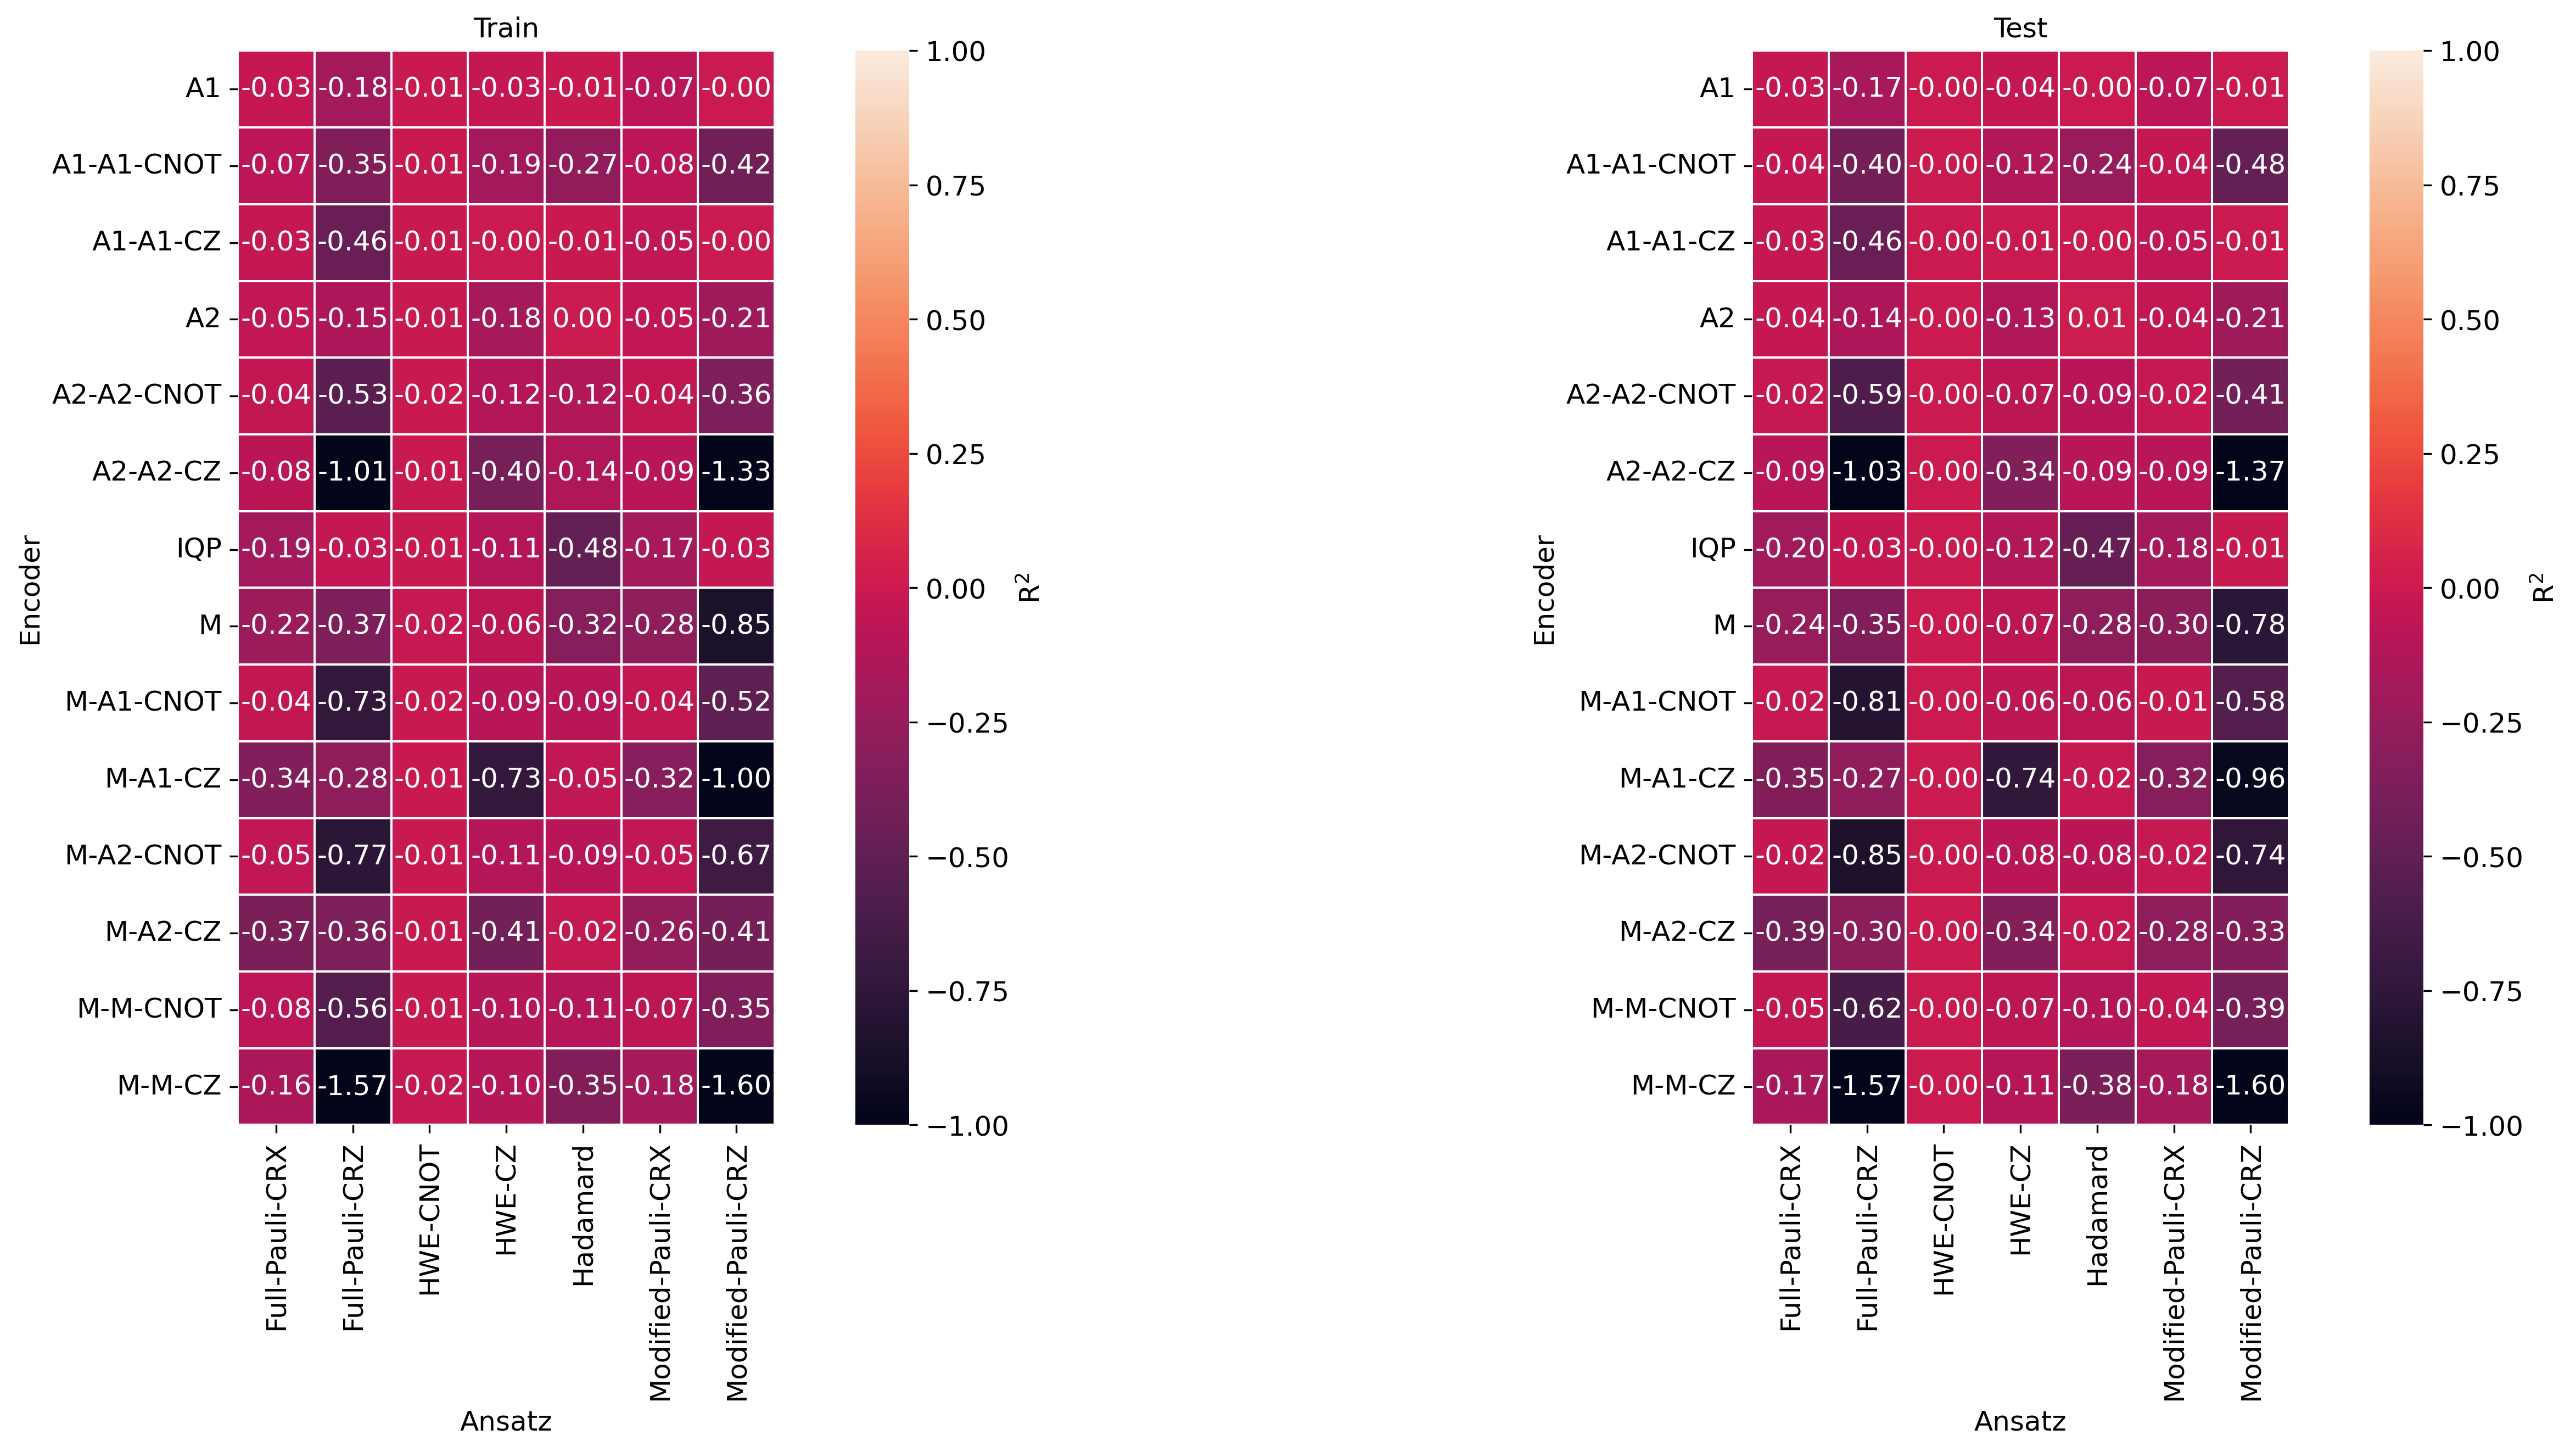
\includegraphics[width=\linewidth]{../images/BSE/sixteenqubit/BSE_heatplots}
		\caption{}
		\label{fig:16BSE_heatplots}
	\end{subfigure}
	\hfill
	\begin{subfigure}[b]{0.49\textwidth}
		\centering
		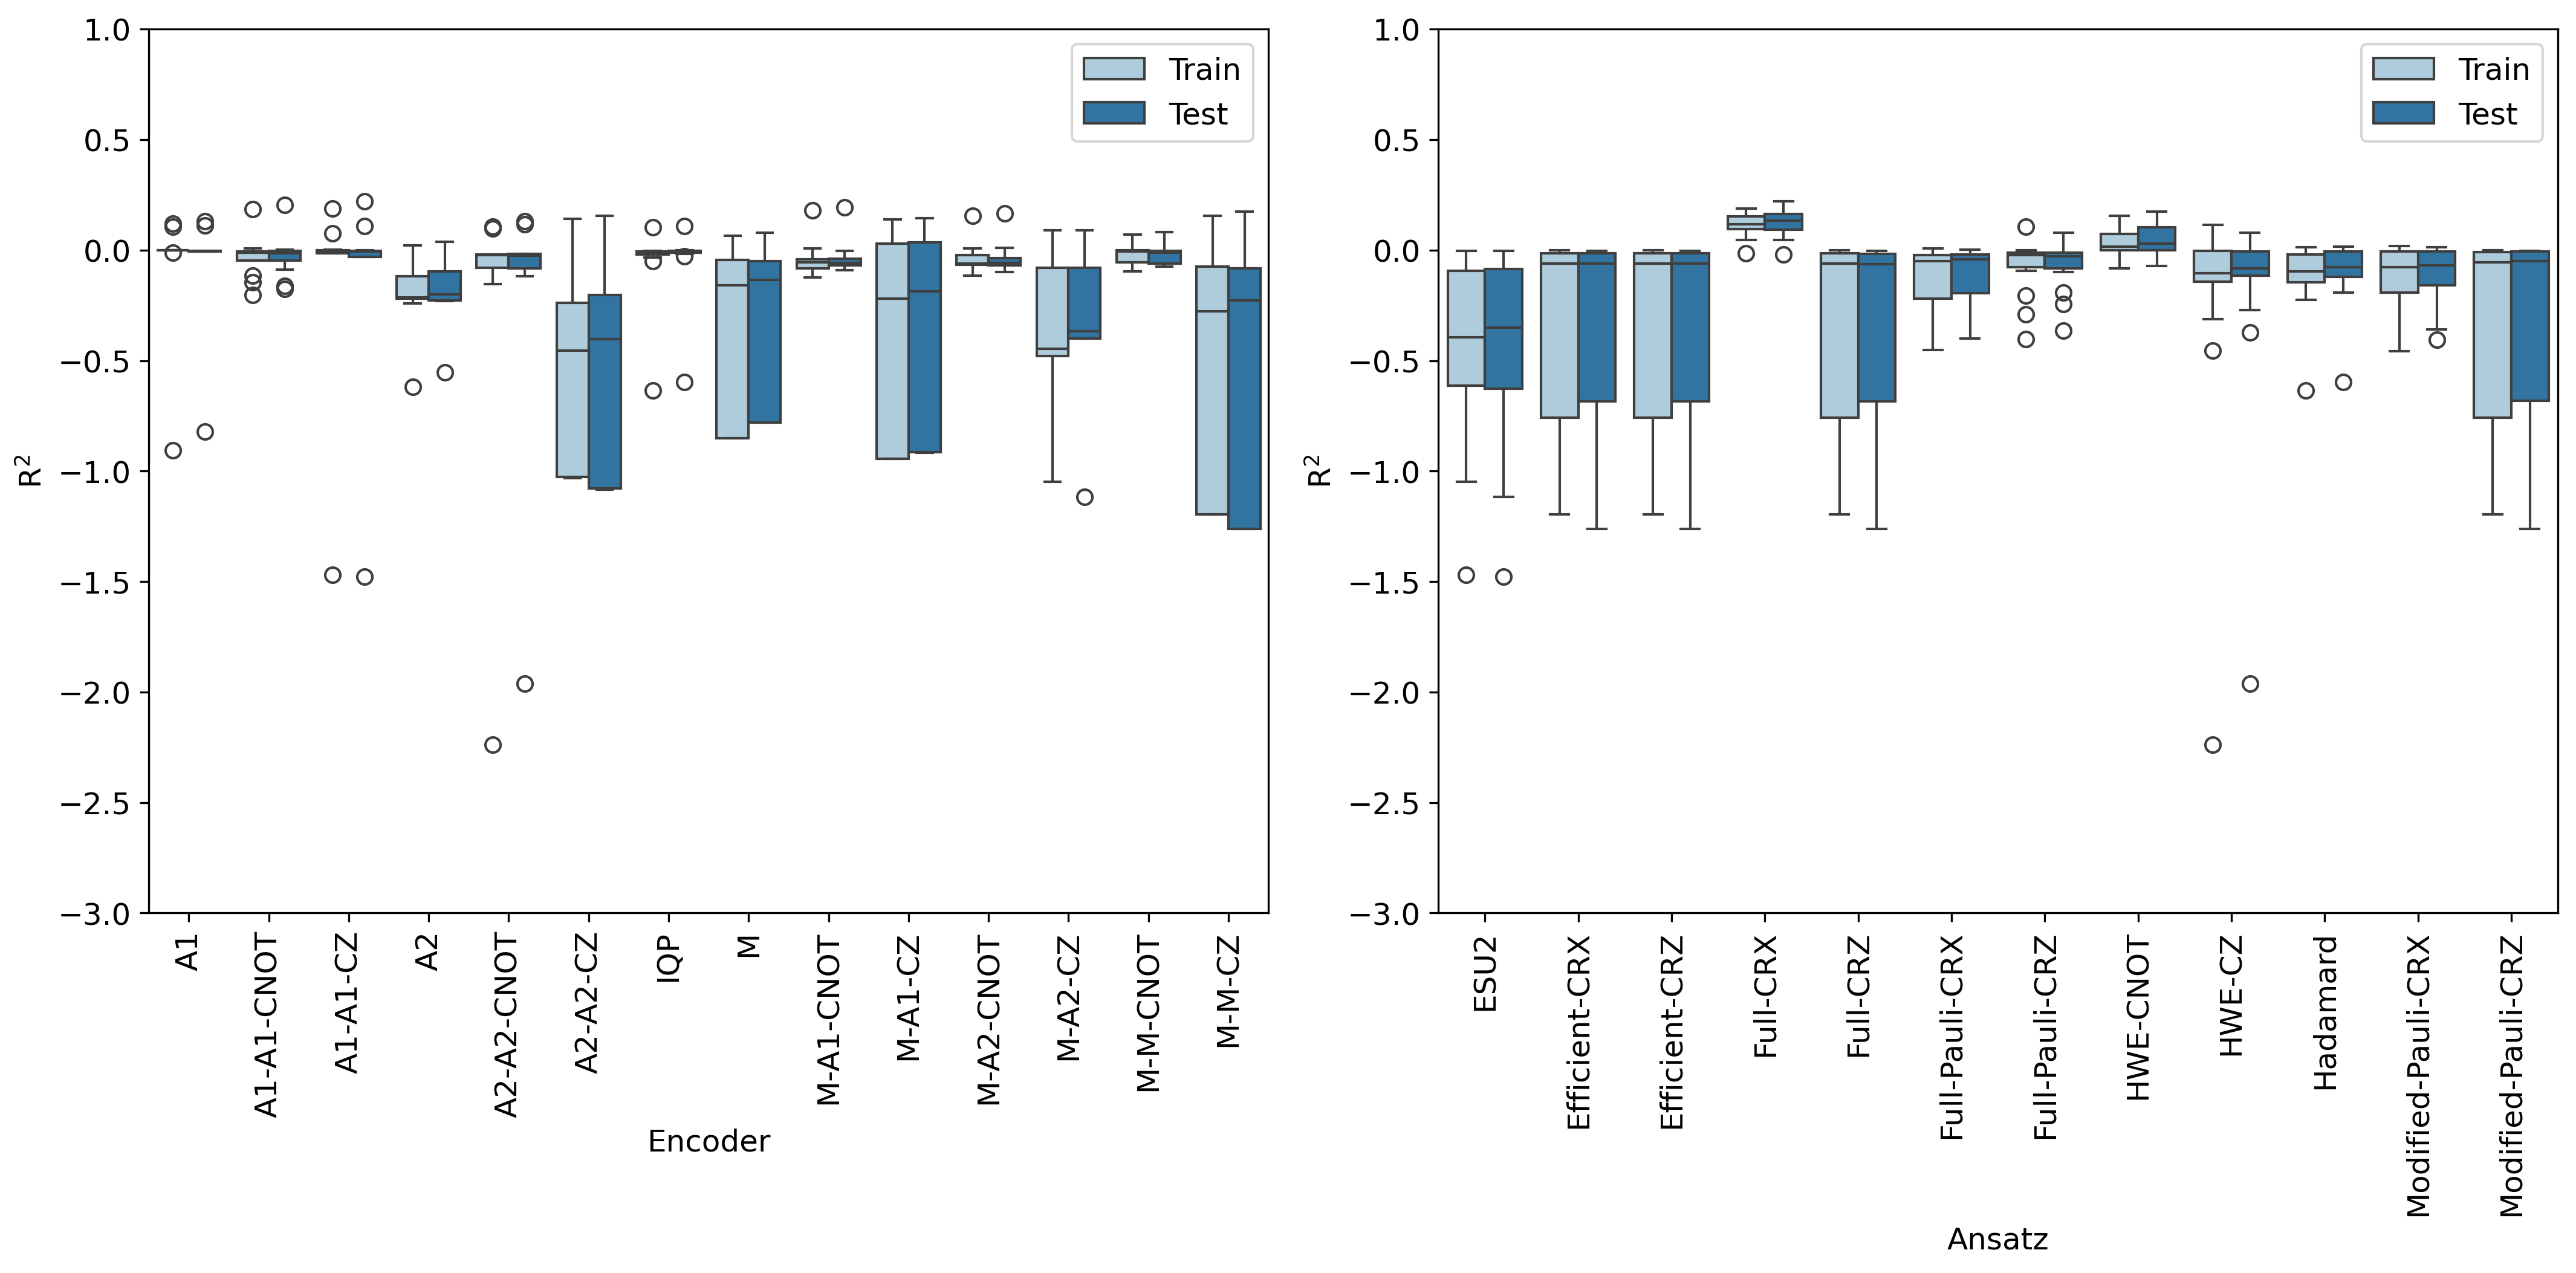
\includegraphics[width=\linewidth]{../images/BSE/fivequbit/BSE_boxplots}
		\caption{}
		\label{fig:5BSE_boxplots}
	\end{subfigure}
	\hfill
	\begin{subfigure}[b]{0.49\textwidth}
		\centering
		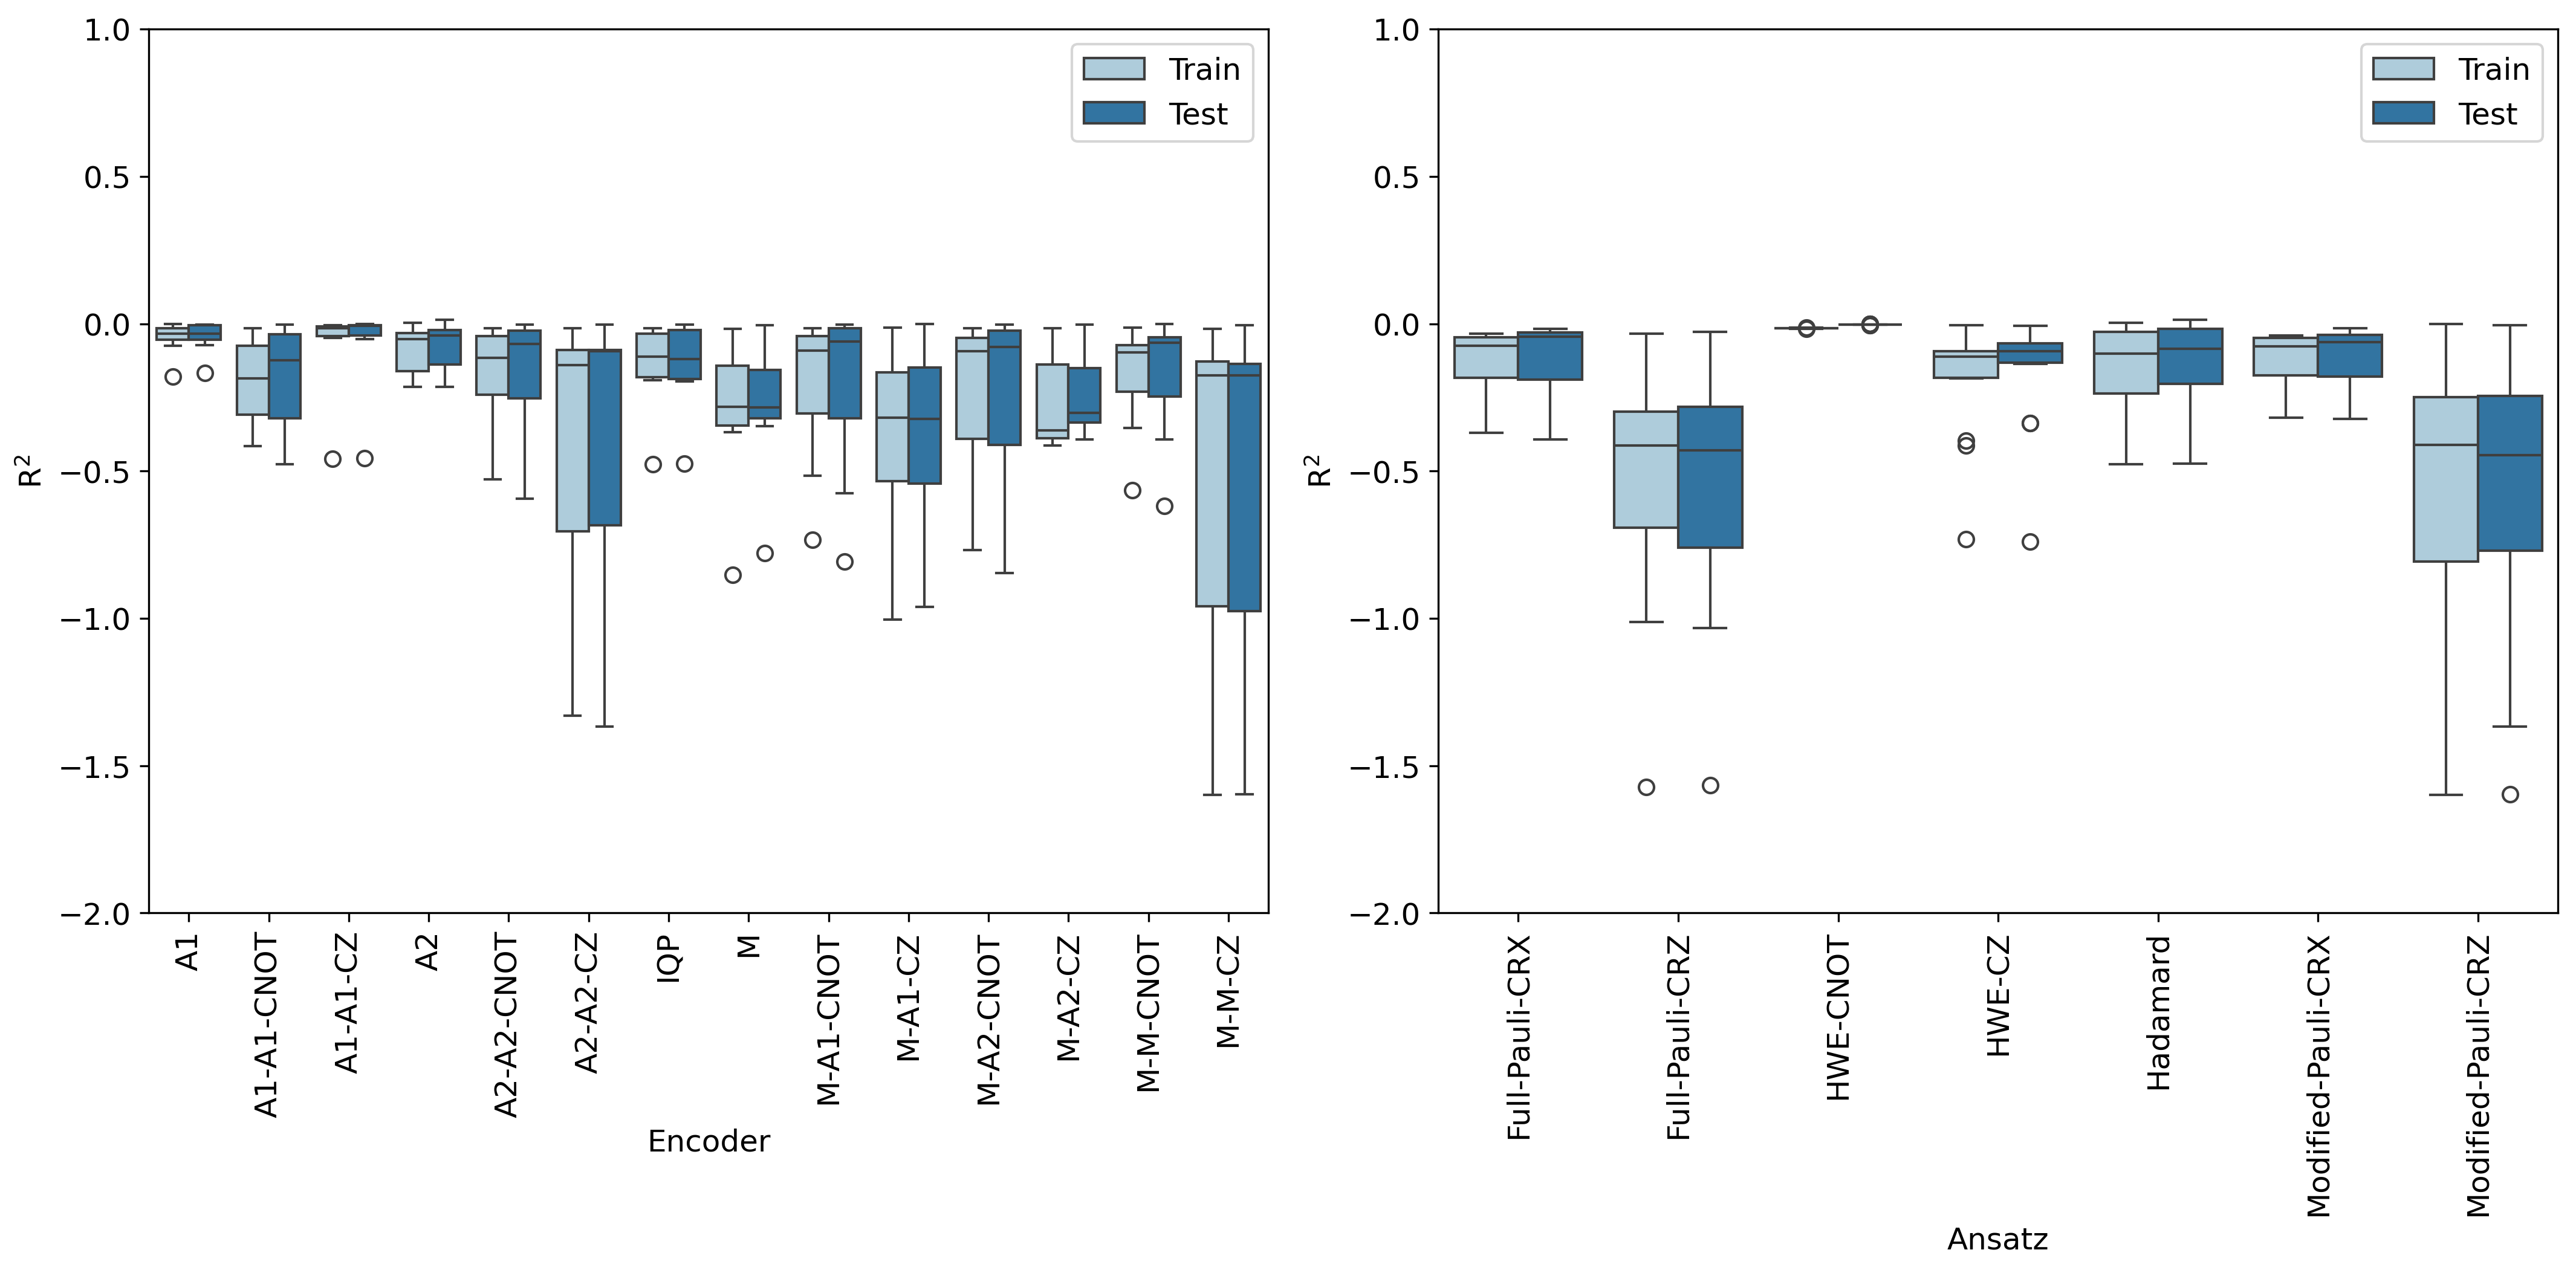
\includegraphics[width=\linewidth]{../images/BSE/sixteenqubit/BSE_boxplots}
		\caption{}
		\label{fig:16BSE_boxplots}
	\end{subfigure}
	\caption{The model performance (in R$^{2}$) of the 168 parameterized quantum circuits for BSE49 using (a) 5 and (b) 16 qubits, where the x-axis denotes the ansatz and the y-axis denotes the encoders. Box plots are used to highlight the general performance of the encoder (left) and ansatz (right) circuits for the (c) 5 and (d) 16 qubit BSE49 models.}
	\label{fig:BSEboxandheat}	
\end{figure}

Following the evaluation of the 168 PQCs using the BSE49 dataset, we used a reduced set of 98 PQCs for the DDCC dataset.
Fig. \ref{fig:ddccheatplots} highlights the improved performance of the PQCs on the DDCC dataset over the BSE49 dataset, where the R$^{2}$s of the training set have a minimum, mean, maximum, and standard deviation of -2.1302, -0.3050, 0.6191, and 0.4422, respectively.
While the R$^{2}$s of the test set have a minimum of -2.1007, a mean of -0.3046, a maximum of 0.6184, and a standard deviation of 0.4411.
The best encoder-ansatz pair is A2{\_}HWE-CNOT with R$^{2}$s of 0.6191 and 0.6184, for the training and test sets, respectively.
We found that the PQCs offer better model performance when run on the DDCC dataset, with A1 offering the best average performance of the encoders with an R$^{2}$ of 0.0163 for the training set and 0.0183 for the test set (Fig. \ref{fig:ddccboxplots} left).
Like the 16 qubit BSE49 data, the best ansatz layer is HWE-CNOT (Fig. \ref{fig:ddccboxplots} right).
Unlike the 16 qubit BSE49 data, HWE-CNOT offers a training and test set R$^{2}$ of 0.2817 and 0.2853, respectively.
Overall, the DDCC models offer more accurate models, with less overfitting, when compared to the BSE49 models.

\begin{figure}[H]
	\centering	
	\begin{subfigure}[b]{0.49\textwidth}
		\centering
		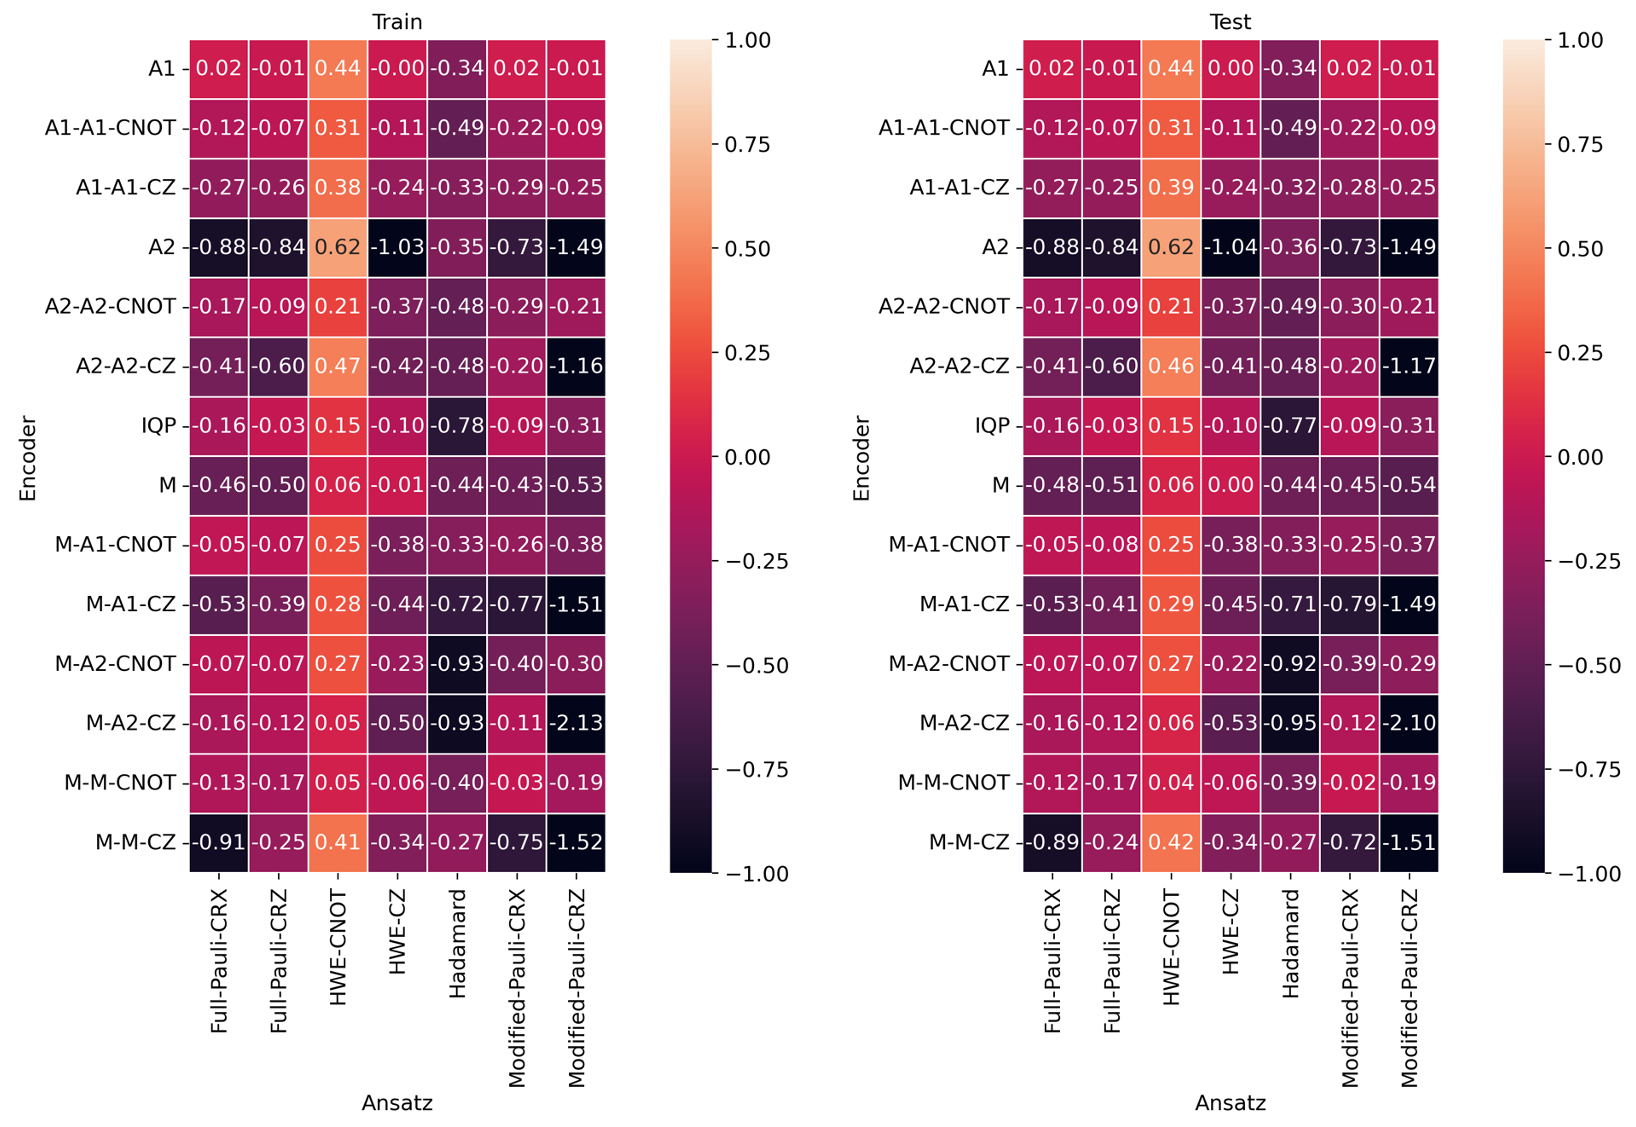
\includegraphics[width=\linewidth]{../images/DDCC/DDCC_heatplots}
		\caption{}
		\label{fig:ddccheatplots}
	\end{subfigure}
	\hfill	
	\begin{subfigure}[b]{0.49\textwidth}
		\centering
		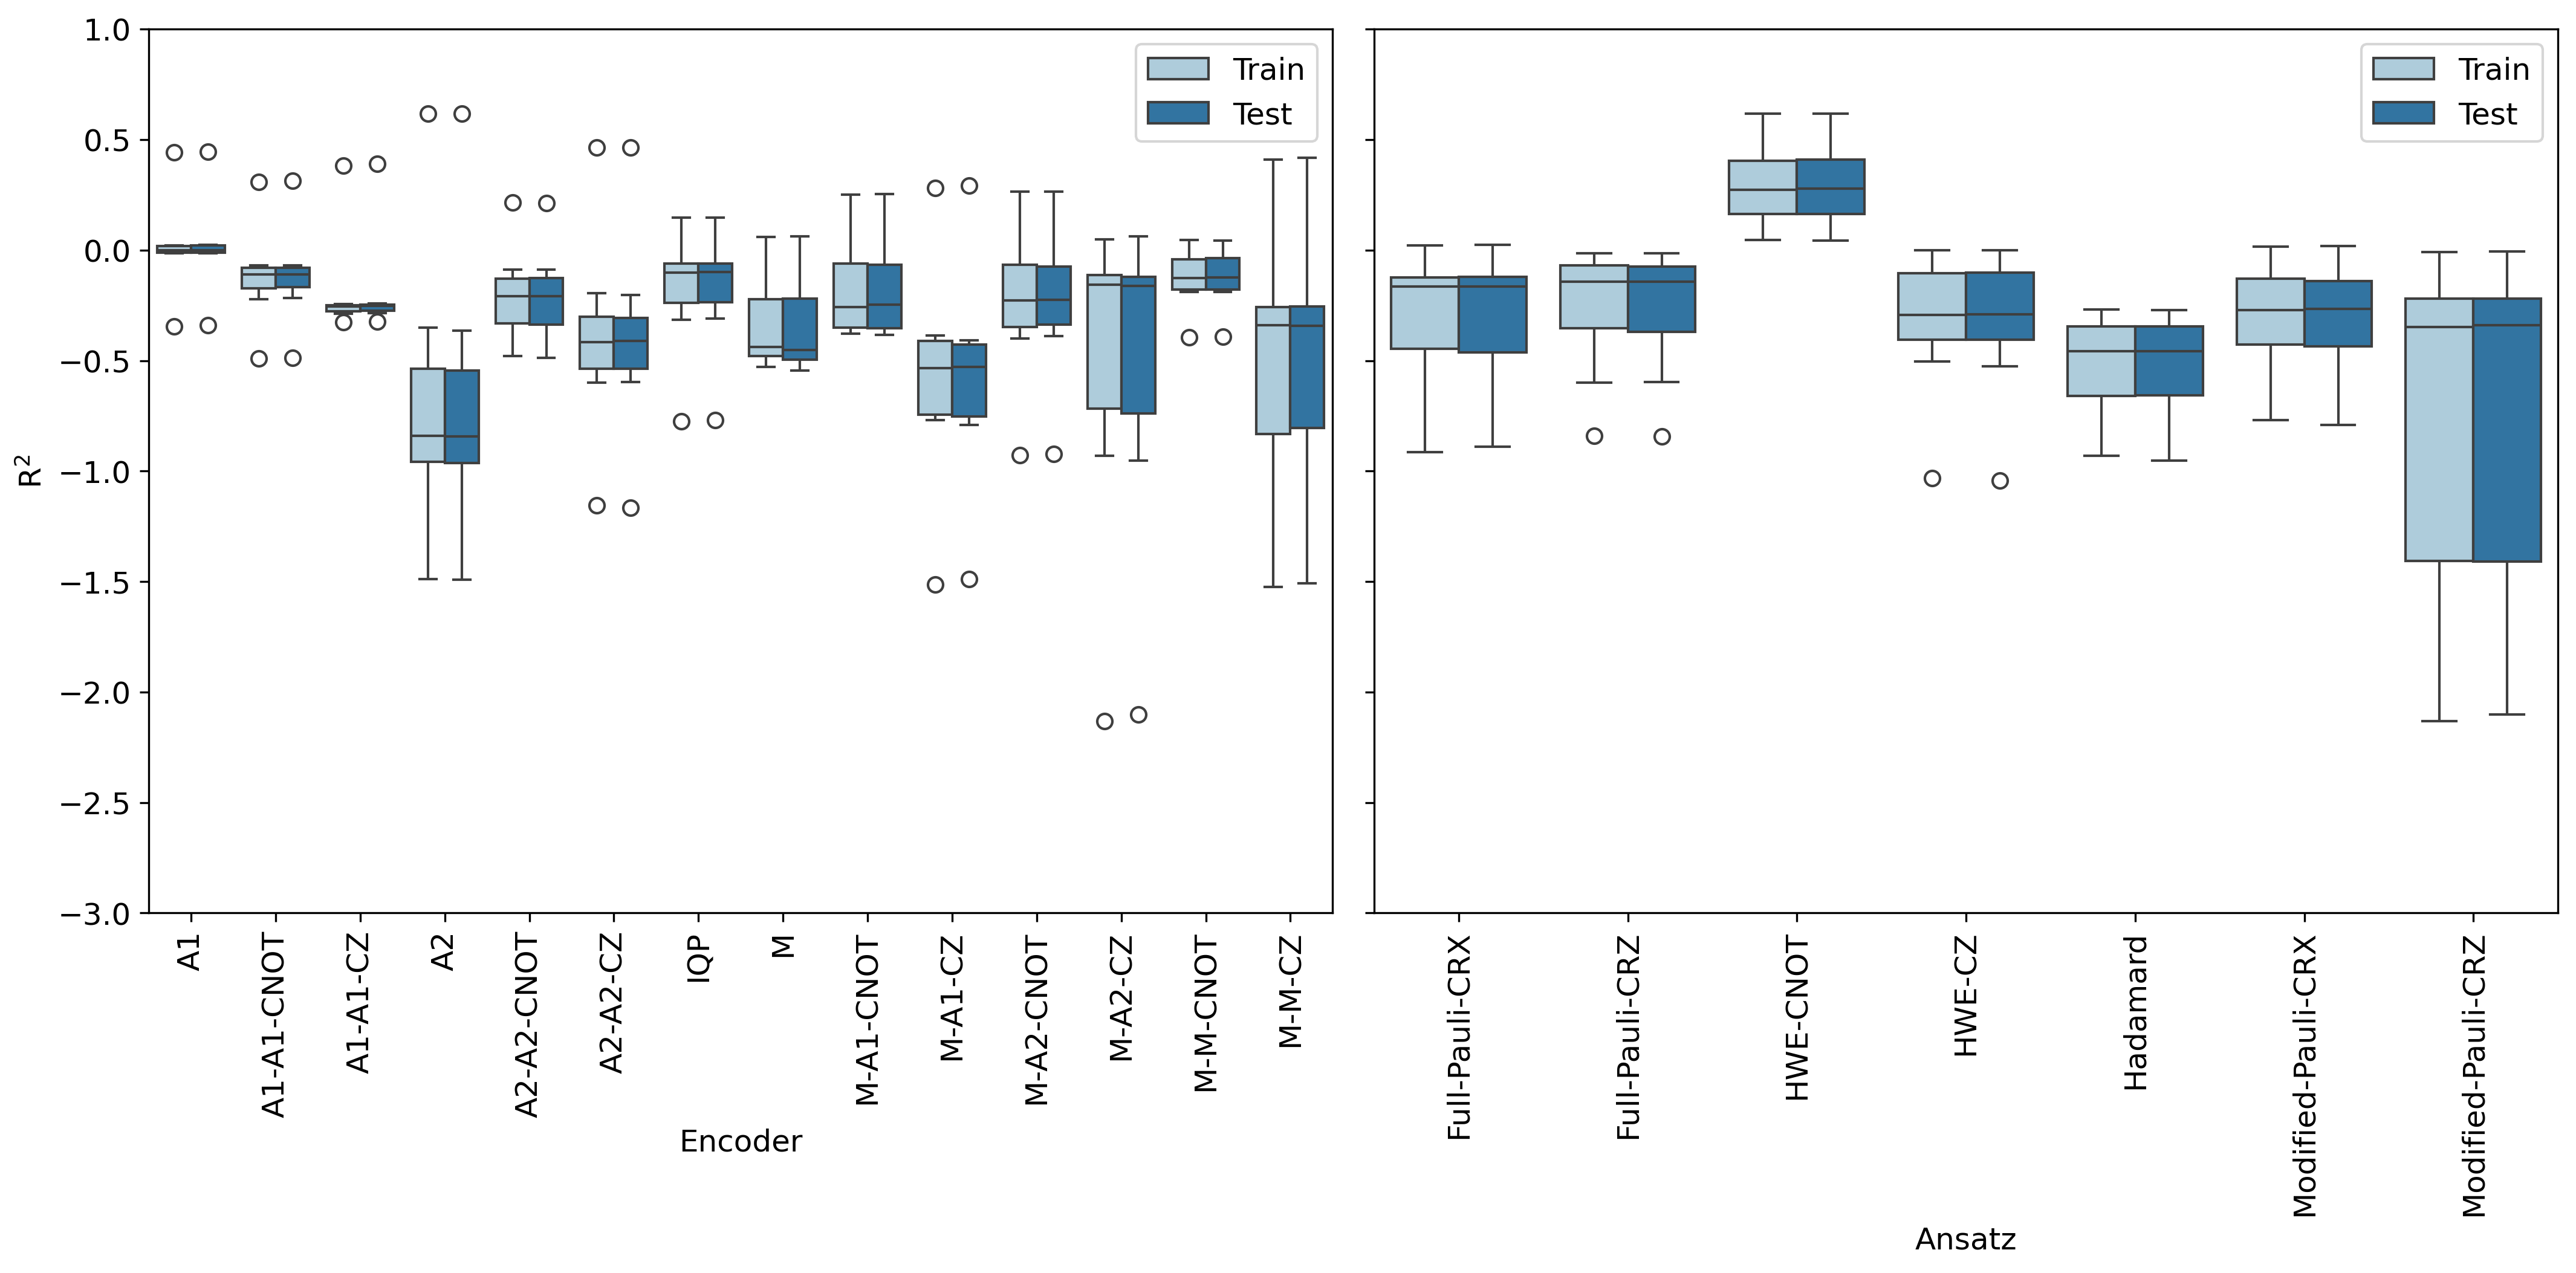
\includegraphics[width=\linewidth]{../images/DDCC/DDCC_boxplots}
		\caption{}
		\label{fig:ddccboxplots}
	\end{subfigure}
	\caption{(a) Heat maps for the 98 PQCs using the DDCC data set for the training (left) and test set (right). (b) Shows box plots for the encoder (left) and ansatz (right) circuits.}
	\label{fig:ddcc_all_analysis}	
\end{figure}


After analyzing the initial set of PQCs using the BSE49 and DDCC datasets, we examine how increasing the re-upload depth (RUD) and number of ansatz layers (AL) affects model performance.
For the BSE49 data, we examine RUDs of $k=\{1,3,5\}$ and for the ALs $v=\{1,3,5\}$.
We examine this data in two ways, the first is a simple line plot, shown in Fig. \ref{fig:bse5RUDAL_lineplot}, where the number of ALs and the RUD layers are plotted on the x-axis, the y-axis denotes the model accuracy in R$^{2}$, and the training set is denoted in light blue, while the test set is shown in dark blue.
The second is by analyzing the regression parity plots, Fig. \ref{fig:BSE5_distribution_parity}, with the addition of kernel density estimation (KDE) plots on the axes to highlight the distributions of the values.
Overall, for M-M-CZ{\_}HWE-CNOT using the BSE49 dataset, increasing the number of ALs and RUD offer negligible improvements over the base model, which as R$^{s}$ of 0.16 and 0.17 for the training and test set, respectively.
The model with the best R$^{2}$ for the training set is the model initial model using an AL of 1 and RUD 1, while the model with the best R$^{2}$ for the test set uses an AL of 1 and RUD of 5 where the R$^{2}$ is 0.18.
When we analyze the distributions in \ref{fig:BSE5_distribution_parity}, we find that the reference target values have a wide distribution, ranging from 9.3800 to 177.2400 kcal/mol with a standard deviation of 27.4877 kcal/mol.
For the predicted values, all of the models struggle with predicting an accurate range, where the model with the worst spread is AL=3/RUD=1 with a minimum of 67.6736 kcal/mol, maximum of 115.6791 kcal/mol, and standard deviation of 6.7346 kcal/mol.
The best model, regarding the spread of the predicted data, is the AL=1/RUD=5, with a minimum of 49.8978 kcal/mol, a maximum of 127.8078 kcal/mol, and standard deviation of 14.0201 kcal/mol. 
Overall, all models, regardless of the number of ALs and RUD, tend to regress towards the mean value of the reference data, 90.6916 kcal/mol.

Unlike the 5 qubit BSE49 data, we see that when we increase the number of ALs and RUD, A2{\_}HWE-CNOT with the DDCC dataset, shows improved model performance (Figs. \ref{fig:ddccRUDAL_lineplot} and \ref{fig:ddccdistribution_parity}).
For this dataset, we go beyond ALs and RUDs of 5 due to the initial improvements shown as both values increased.
Fig. \ref{fig:ddccRUDAL_lineplot} highlights an interesting trend whereas the number of ALs increases the model performance increases from R$^{2}$s of 0.62 to R$^{2}$s of $\approx 0.80$, for both the training and test sets.
For the RUD, the R$^{2}$s show marginal improvements at $k=5,9$ while showing increased performance for $k=3,5$. 
Overall, the best model for A2{\_}HWE-CNOT with the DDCC dataset is the model with an AL of 5 and RUD of 1.
This is highlighted in Fig. \ref{fig:ddccdistribution_parity}, where we see that the distribution of the predicted target values is closer to the spread of the reference values than the initial model with AL=1/RUD=1.





\begin{figure}[H]
	\centering	
	\begin{subfigure}[b]{0.49\textwidth}
		\centering
		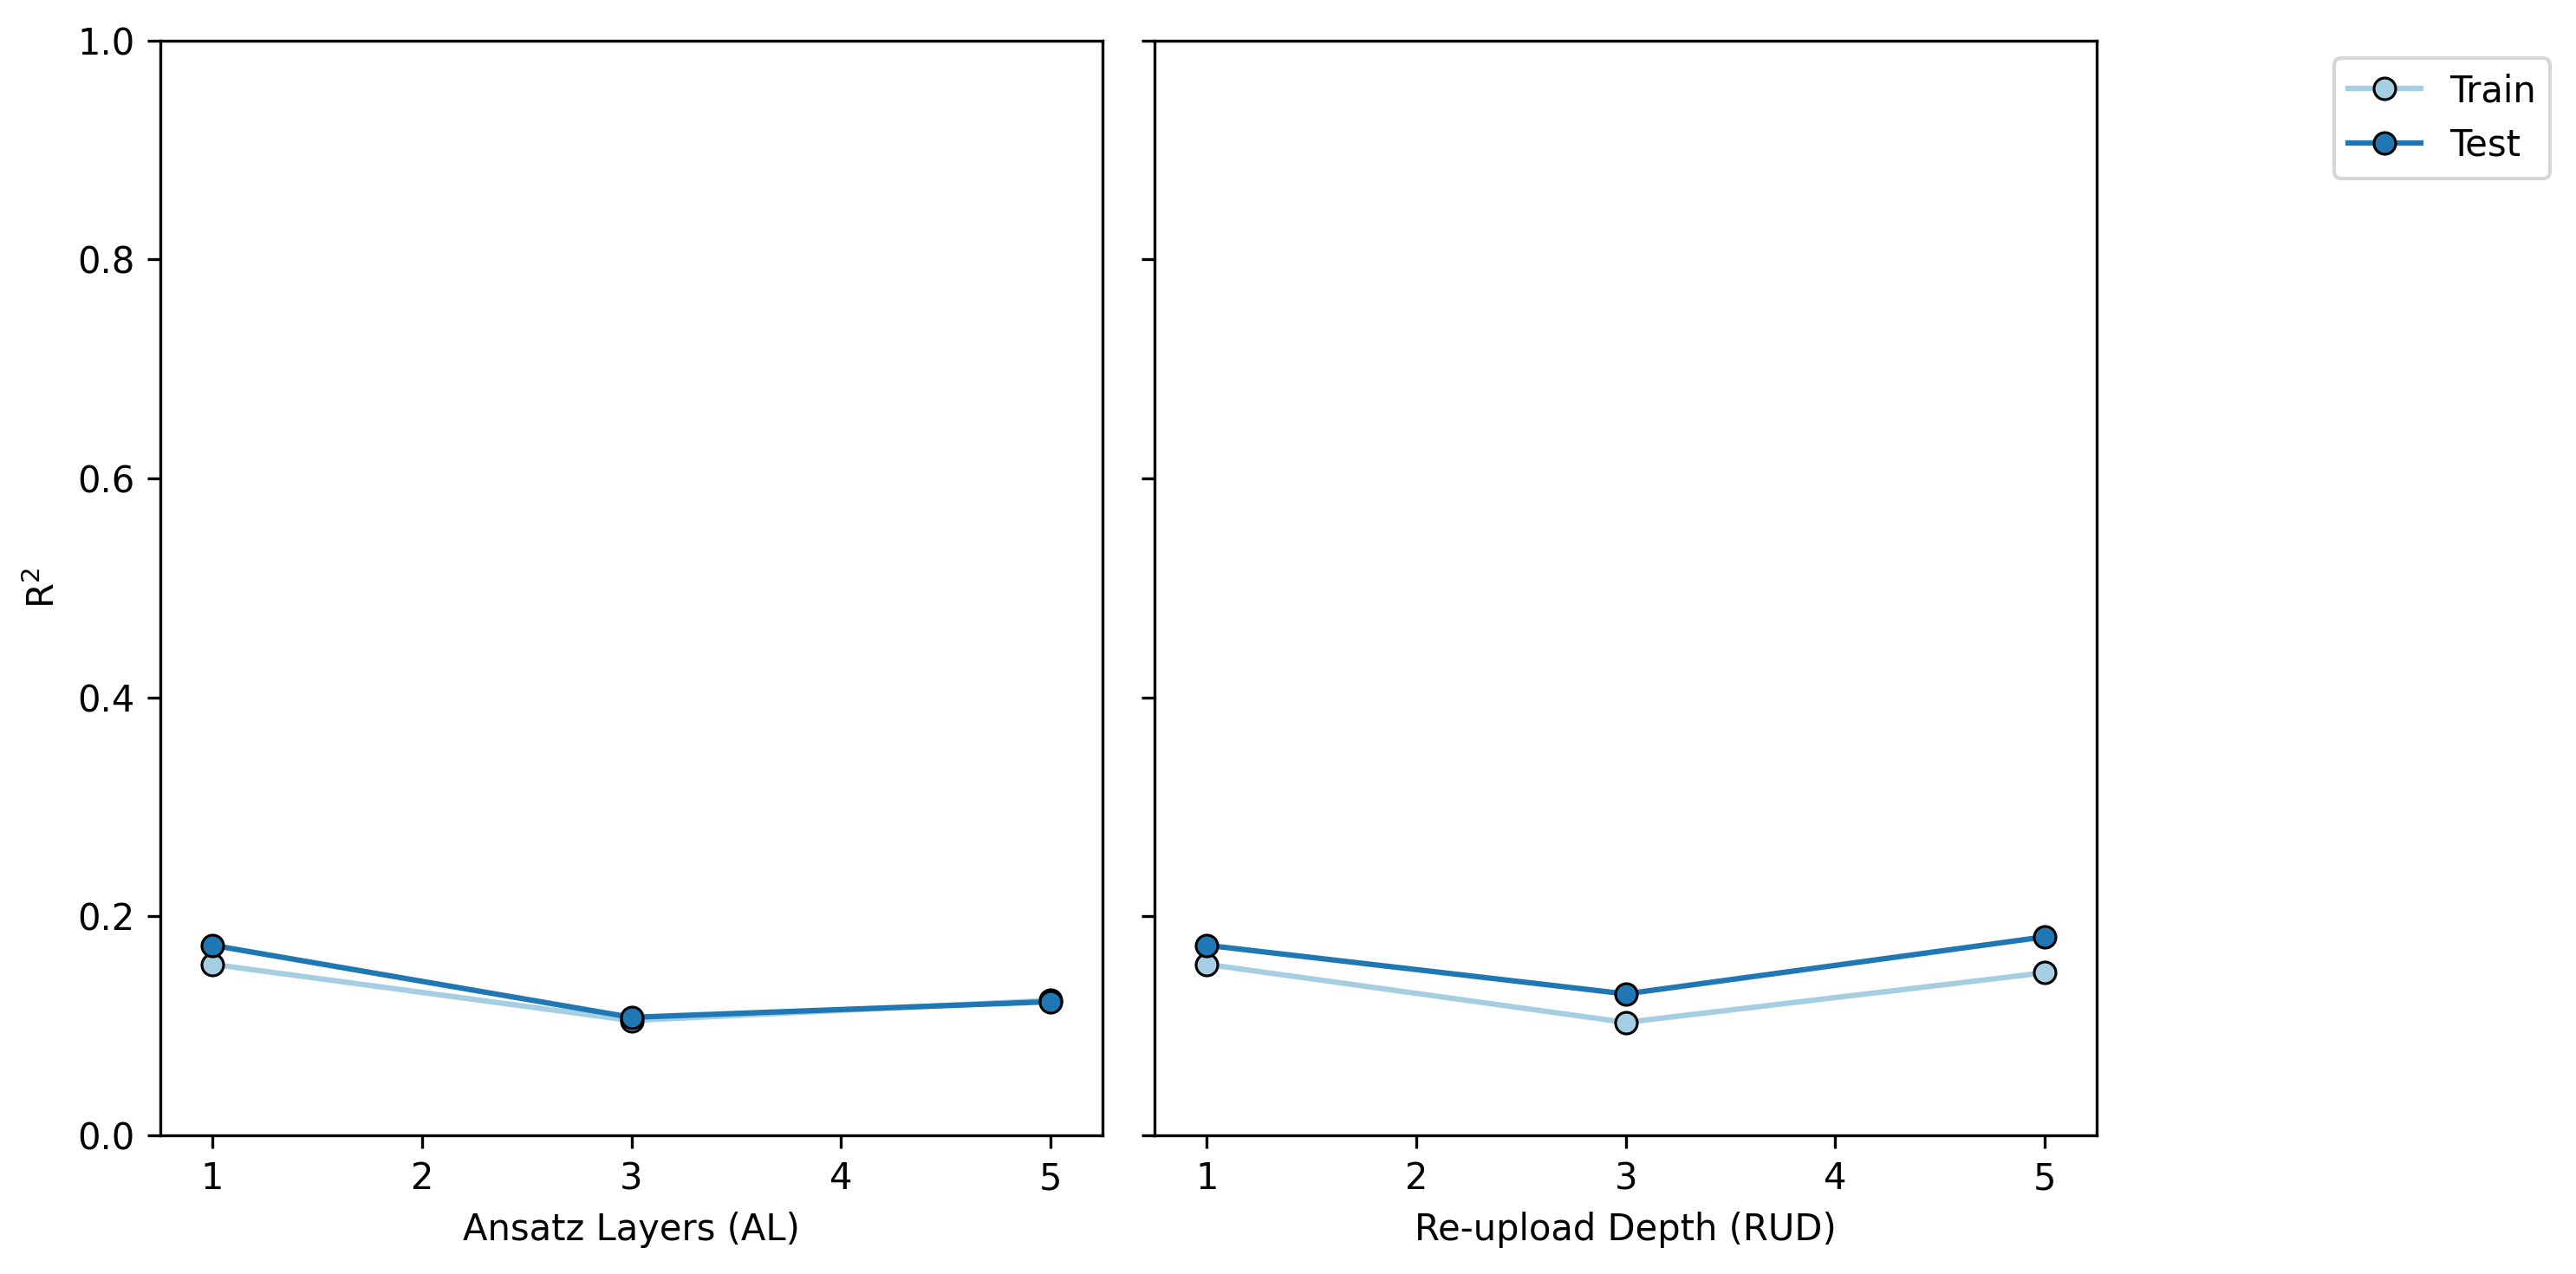
\includegraphics[width=\linewidth]{../images/BSE/fivequbit/BSE5_RUDAL_lineplot}
		\caption{}
		\label{fig:bse5RUDAL_lineplot}
	\end{subfigure}
	\hfill
	\begin{subfigure}[b]{0.49\textwidth}
		\centering
		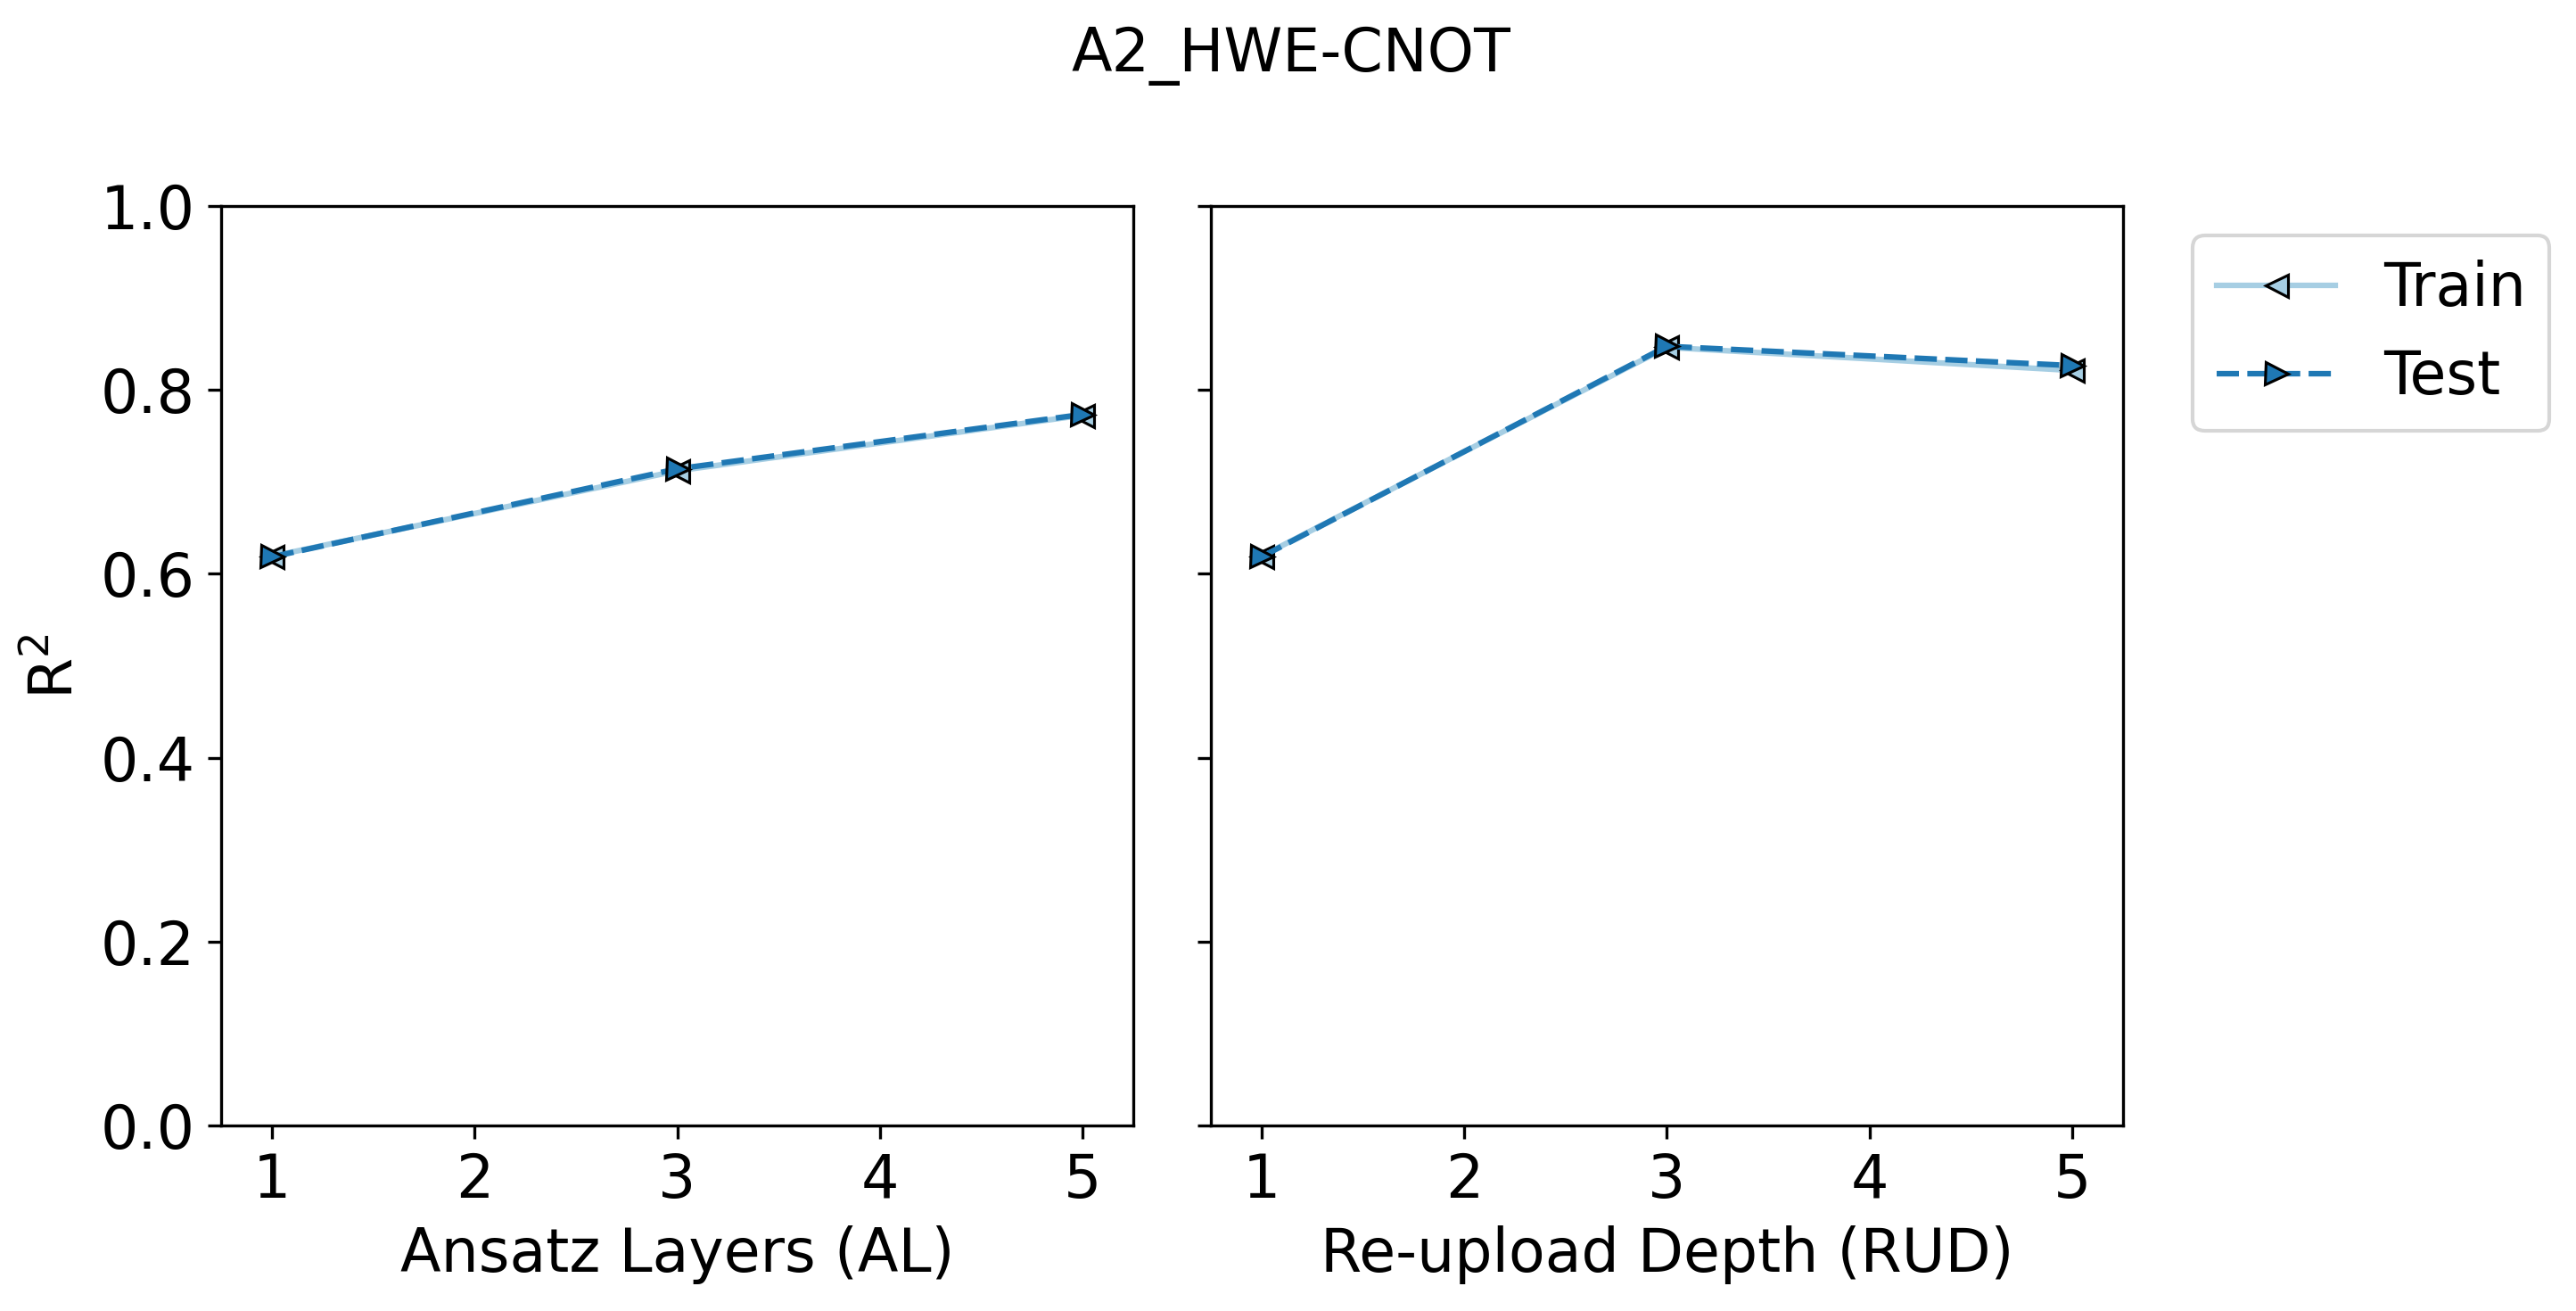
\includegraphics[width=\linewidth]{../images/DDCC/DDCC_RUDAL_lineplot}
		\caption{}
		\label{fig:ddccRUDAL_lineplot}
	\end{subfigure}
	\hfill	
	\begin{subfigure}[b]{0.49\textwidth}
		\centering
		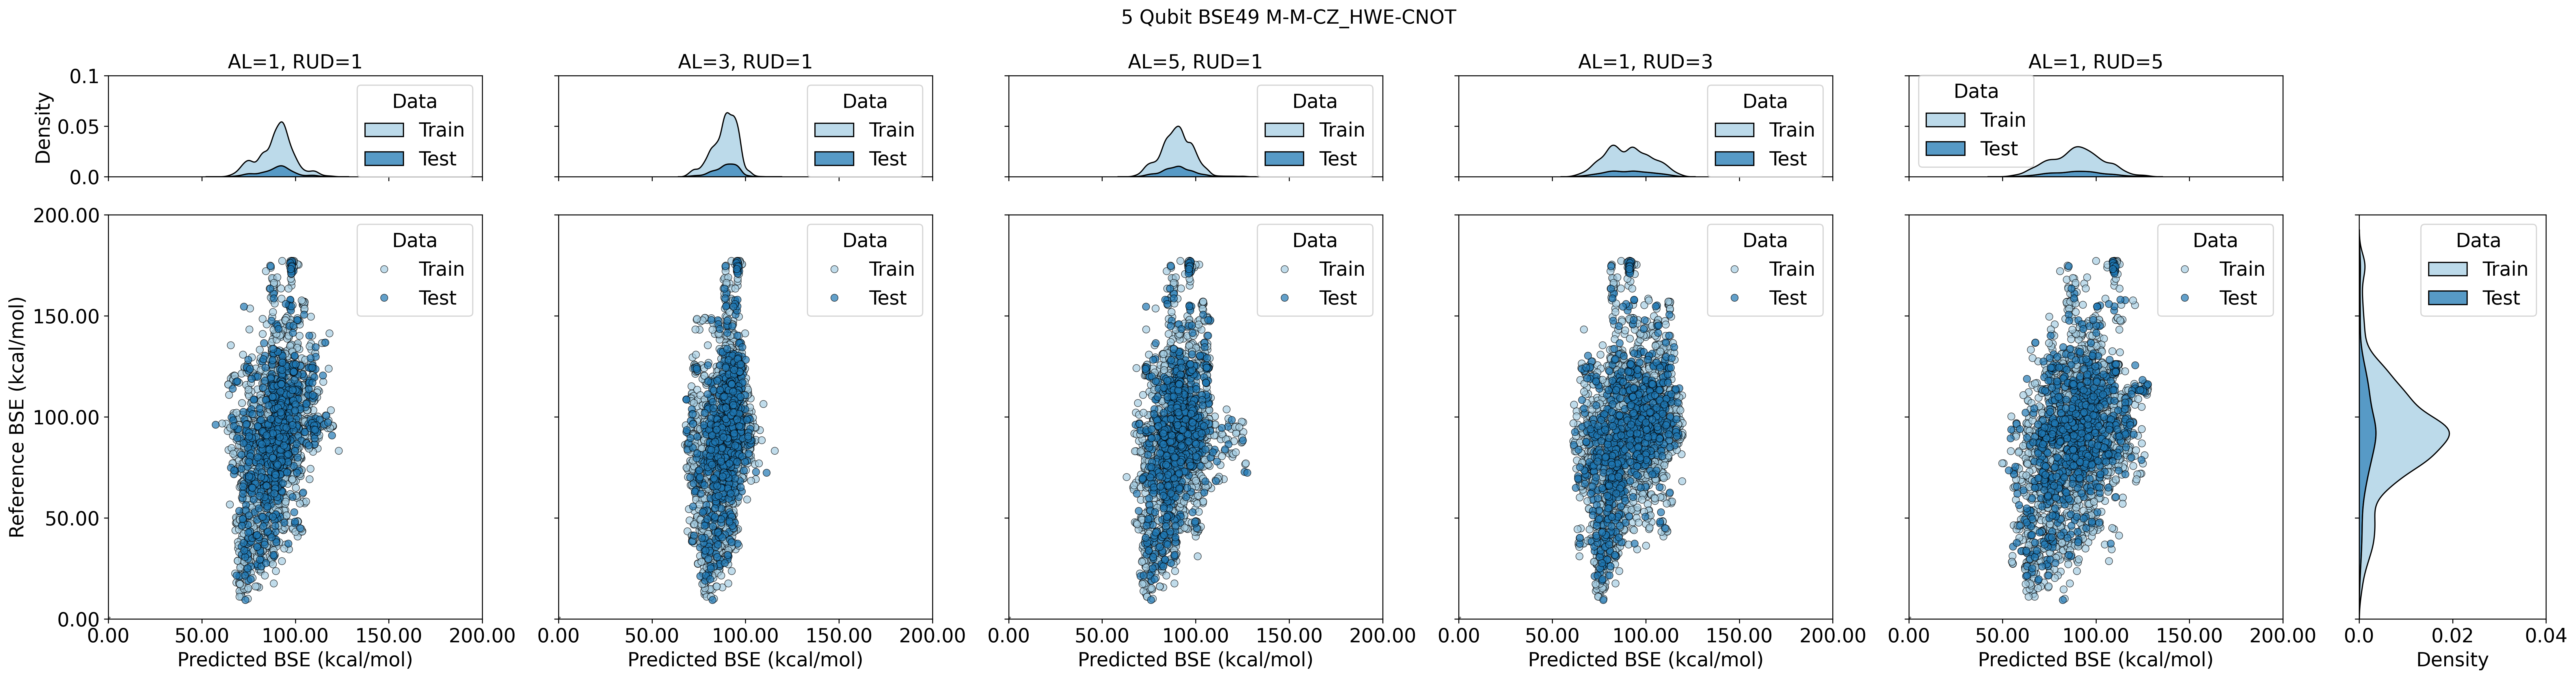
\includegraphics[width=\linewidth]{../images/BSE/fivequbit/distribution_parity}
		\caption{}
		\label{fig:BSE5_distribution_parity}
	\end{subfigure}
	\hfill

	\begin{subfigure}[b]{0.49\textwidth}
		\centering
		\includegraphics[width=\linewidth]{../images/DDCC/distribution_parity}
		\caption{}
		\label{fig:ddccdistribution_parity}
	\end{subfigure}	
	\caption{Line plots to highlight the performance as the number of ansatz layers (AL; left) and re-upload depth (RUD; right) increases for the 5 qubits (a) BSE49 and (b) DDCC data. Additionally, regression parity plots for each AL and RUD are shown for the (c) BSE49 and (d) DDCC data, where the x-axis denotes the predicted target values and the y-axis denotes the reference data.}
	\label{fig:BSE_distribution_parity}	
\end{figure}

Following the analysis of the RUD and number of ALs for both 5 qubit models, we explored claims that PQCs offer better model performance using fewer training points and hyperparameters\cite{schuld_circuit-centric_2020,du_expressive_2020,suzuki_predicting_2020} using learning curves.
We generate the learning curves by varying the number of training points from 10-80\% of the total data while holding the number of test points to 20\% of the total dataset.
In Fig. \ref{fig:learningcurves}, we analyze the effects of the number of training points of the best 5 qubits BSE49 and DDCC circuits, M-M-CZ{\_}HWE-CNOT using a RUD and AL of 1 and A2{\_}HWE-CNOT using a RUD of 
For the BSE49 dataset, using 5 qubits, we found that M-M-CZ{\_}HWE-CNOT offers less overfit models, but offers poorer performance regarding the training and test set R$^{2}$s, as highlighted in Fig. \ref{fig:BSE5_learning_curves}.
Across the learning curve, the \textit{k}-NN model has a mean R$^{2}$s of 0.9998 for the training set and 0.5822 test set, while M-M-CZ{\_}HWE-CNOT has a mean R$^{2}$ of 0.1405 for the training set and R$^{2}$ of 0.136 for the test set.
For M-M-CZ{\_}HWE-CNOT, the training set performance peaks when using 10\% of the training data with an R$^{2}$ of 0.2015, dips to an R$^{2}$ of -0.0172 using 30\% of the training data, and then maintains an R$^{2}$ less than 0.2 for the remaining percentages of the training data.
Unlike the training points, the test reaches peak performance when 70\% of the total data is used in the training set, with a test R$^{2}$ of 0.2064.
The A2{\_}HWE-CNOT circuit on the DDCC dataset has some similarities and differences when compared to M-M-CZ{\_}HWE-CNOT on the BSE49 dataset.
One difference is that A2{\_}HWE-CNOT improves across the learning curve, with maximum R$^{2}$ of 0.8470 and 0.8492 for the training and test sets, respectively.
A common feature between both models is that the classical models outperform the PQCs in both cases, but with the DDCC dataset, the classical models do not exhibit overfitting and have R$^{2}$s greater than 0.98 across the full learning curve.




\begin{figure}[H]
	\centering	
	\begin{subfigure}[b]{0.49\textwidth}
		\centering
		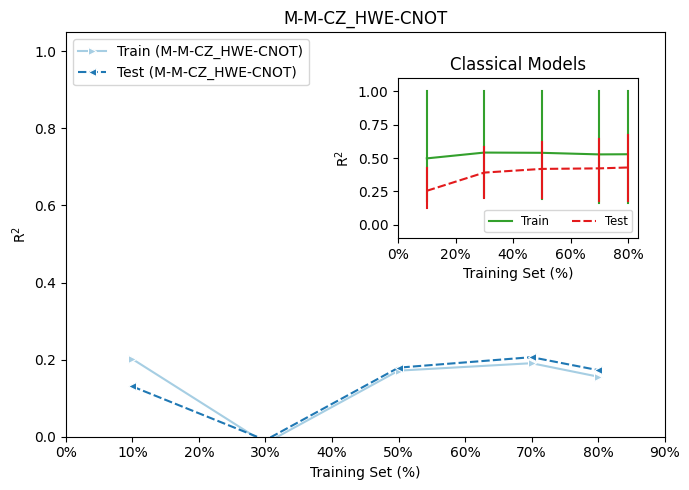
\includegraphics[width=\linewidth]{../images/BSE/fivequbit/BSE_learningcurve}
		\caption{}
		\label{fig:BSE5_learning_curves}
	\end{subfigure}	
	\hfill
	\begin{subfigure}{0.49\textwidth}
		\centering
		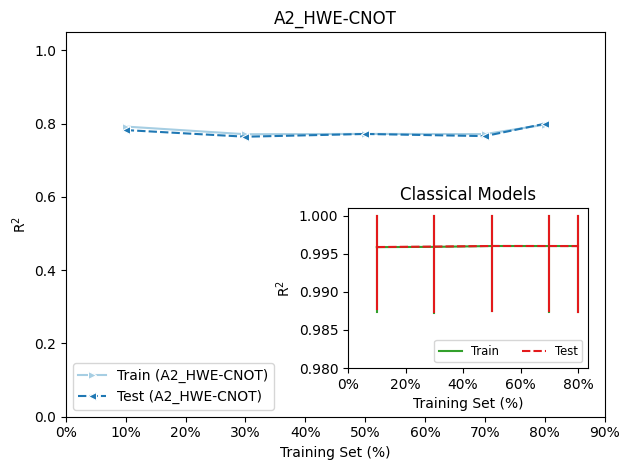
\includegraphics[width=\linewidth]{../images/DDCC/DDCC_learning_curves}
		\caption{}
		\label{fig:ddcclearningcurves}
	\end{subfigure}
	\caption{Learning curves for the (a) BSE49 database using the M-M-CZ{\_}HWE-CNOT circuit and (b) the DDCC dataset using the A2{\_}HWE-CNOT circuit. The x-axis denotes the percentage of training points, while the test set is held to 20\% of the total data. The y-axis denotes the R$^{2}$ of the training and test learning curves. Inlay plots show the training and test data for the classical models examined, where the bottom error bar denotes the minimum value, the line is the mean value, and the top error bar is the maximum value.}
	\label{fig:learningcurves}
	
\end{figure}

Following the evaluation of the learning curves, we decided to only run the A2{\_}HWE-CNOT circuit on real quantum hardware.
Before running on the real hardware (\textit{ibm{\_}quebec}), we optimize the number of shots, the resilience level, and optimization using the \textit{FakeQuebec} backend with the \textit{qiskit-aer} plugin.
Based on the results from the observations provided by the state vector learning curves (Fig. \ref{fig:ddcclearningcurves}), along with considerations regarding the computational cost associated with the query time to the IBM Quantum platform, number of training points ($N_{\text{occ}}^{2}N_{\text{virt}}^{2}$ $t_{2}$-amplitudes), along with the potential number of device executions associated with the number of shots, resilience (error mitigation) and optimization levels the total number of training data is reduced from 80\% to 10\% of the total training data.
We validated this assumption using the \textit{ibm{\_}quebec} device using Twirled Readout Error eXtinction (TREX) \cite{van_den_berg_model-free_2022} error mitigation (resilience level 1), an optimization level of 2, with 3072 shots for both 10\%  and 80\% of the training data.
Using one iteration, we found that one iteration using 10\% of the training data took 1824 s of wall time, versus one iteration using 80\% of the training data taking 25004 s of wall time.
For a model that requires 500 or 1000 iterations to train, this would require approximately 145 to 289 days to train an end-to-end model using \textit{ibm{\_}quebec} using 80\% of the training data, versus 10 to 21 days required to train the model containing 10\% of the total data.
While this is still much longer than the classical models, the value of running on real hardware is still a worthwhile experiment to show how these models behave on the current generation of hardware.
 


To efficiently run the DDCC model on \textit{ibm{\_}quebec} the data is split into batches of 4 molecules per sample with 64 $t_{2}$-amplitudes each.
The motivation for batching the data is to reduce the number of circuit executions per primitive unified blocs (PUBs).
We found that for 500 iterations, an optimization level of X, with a resilience level of Y, using Z shots was adequate to reach satisfactory model performance using the \textit{FakeQuebec} backend (\textbf{Update these figures} Figs. \ref{fig:optresfakequebec} and \ref{fig:shotsfakequebec}).
When applied on \textit{ibm{\_}quebec} we found that the models had R$^{2}$s of X and Y, for the training and test set, respectively, and took a total of X QPU time and Y wall time to complete.





Ansaetze analysis \cite{sim_expressibility_2019}
``In particular, a substantial improvement in performance of two-qubit gates in a ring or all-to-all connected arrangement, compared to that of those on a line, is observed.''

``Furthermore, improvement in both descriptors is achieved by sequences of controlled X-rotation gates compared to sequences of controlled Z-rotation gates.''

``investigated how expressibility “saturates” with increased circuit depth, finding that the rate and saturated value appear to be distinguishing features of a PQC''




level 1 readout error mitigation and measurement twirling using Twirled Readout Error eXtinction (TREX) \cite{van_den_berg_model-free_2022}
level 2 level 1 + gate twirling and zero noise extrapolation (ZNE)\cite{kandala_error_2019,li_efficient_2017,temme_error_2017}


For the circuits we perform experiments with, there exists a quantum advantage regarding the time complexity of training the quantum circuit classically versus on the quantum hardware. 
There is a very big caveat that must be addressed regarding the DDCC dataset.
Classically the DDCC method can be efficiently optimized in $\mathcal{O}(n)$ to $\mathcal{O}(t \log n)$ time, versus the quantum algorithm that would require $\mathcal{O}(n 2^{2m})$ time.

\begin{table}[h!]
	\centering
	\small
	\begin{tabular}{|c|c|c|c|}
		\hline
		\textbf{Model} & \textbf{\# of Trainable Parameters} & \textbf{\# of Two-Qubit Gates} & \textbf{Circuit Depth} \\
		\hline
		A2\_HWE-CNOT & \(3nvk\) & \(nvk\) & \(vnk + 3vk + 2kl\) \\
		\hline
		M-M-CZ\_HWE-CNOT & \(3nvk\) & \(2nkl + nvk\) & \(2nkl + 2kl + nvk + 3vk\) \\
		\hline
		Linear, Ridge, Lasso, ElasticNet & \(n + 1\) & --- & --- \\
		\hline
	\end{tabular}
	\caption{Comparison of models concerning parameter count, two-qubit gate count, and circuit depth.}
\end{table}

\section{Conclusion}
Quantum advantage in terms of computational complexity but not in model performance?



PQCs for the BSE49 and DDCC datasets do not exhibit an advantage concerning model accuracy, the number of training points, or the time to train the models.
Poor performance on the BSE49 dataset could be explained by the feature space reduction, we are compressing the feature space from 2048 to 5 features (structure-based ML reps. require more features than physics-based reps.)
While the physics-based feature set of DDCC outperforms the structure-based feature set of BSE49, DDCC requires too many device executions to be useful in the current generation of devices
For practitioners of quantum chemistry, who work on machine learning-related tasks, like Viki and me, several options exist:
Use hybrid classical-quantum machine learning approaches to exploit entanglement on the QPU, while using a CPU/GPU/TPU for efficient classical tasks
Classical machine learning assisted quantum computing (like I have proposed for a DDCC-LUCJ project for two undergraduates for summer 2025)
Using distributed QML to maintain short circuit depths, while increasing the number of features
Explore molecular representations designed for QML (e.g., BSE49 is a classic-in/quantum-out case)
Stick to quantum-in/quantum-out approaches (e.g., DDCC falls into this category, but could this be reformulated to better exploit the QPU?)

\textcolor{blue}{DDCC Discussion points}
\begin{itemize}
	\item Using multiple feature encoding qubits\cite{suzuki_predicting_2020} is unfeasible with DDCC due to the number of samples
	\item DDCC is a \textit{trivial} task for classical ML (long time to train QML)
	\item It should also be noted that the majority of the $t_{2}$-amplitudes will be centered near zero since the $t^{ab}_{ij}$ tensor will contain many small contributions. Models that exclude small amplitudes, such as those found in Ref\cite{pathirage_exploration_2024}, could be used for increased performance but are out of the scope of this work.
\end{itemize}

\section{Acknowledgements}
We would like to acknowledge the Government of Canada’s New Frontiers in Research Fund (NFRF), for grant NFRFE-2022-00226, and the Quantum Software Consortium (QSC), financed under grant \#ALLRP587590-23 from the National Sciences and Engineering Research Council of Canada (NSERC) Alliance Consortia Quantum Grants.
This research was enabled in part by support provided by IBM Quantum via the Quantum Software Consortium and the Digital Research Alliance of Canada.
The authors would also like to acknowledge Aviraj Newatia, who provided valuable insights with preliminary results excluded from this work.
[Some things were running on the MSRG cloud... do we need to cite the funders of our cloud???]
[Viki: Did Nick have any special undergrad funding?]

\bibliography{achemso-demo}

\end{document}
